\chapter{Results}
\label{chap:results}

All experiments conducted are about assembling target polyominoes with the use of our global planner (\autoref{chap:global}).
In \autoref{sec:AFN} we analyze the effect of increasing polyomino size on planning time, rotational cost and other global planner characteristics mentioned in \autoref{sec:global_complex}.
The polyominoes used for this experiment are randomly generated, but we also evaluate the construction of manually designed polyominoes in \autoref{sec:AFTS}.
With manually designed polyominoes, we can specifically test the assembly of targets with caves or holes, varying widths and heights, or different patterns of red and blue cubes. 
Furthermore, we experiment with different workspace sizes and aspect ratios in \autoref{sec:AFBS} and how the ratio of red and blue cubes affect the assembly of straight line polyominoes in \autoref{sec:AFNR}.

\paragraph{Option Sorting Strategies}
We conducted all experiments with the three option sorting strategies from \autoref{sec:connect_options}:
\begin{enumerate}
	\item Minimal Distance (MIN DIST)
	\item Grow Largest Component (GROW LARGEST)
	\item Grow Smallest Component (GROW SMALLEST)
\end{enumerate}

\paragraph{Instance Generation}
Random polyominoes and initial configurations were created with a seed-based pseudorandom number generator, to make experiments reproducible.
The option sorting strategies are applied to the same set of seeds to make the results comparable.
When an initial configuration is randomly generated, the number of red and blue cubes matches with the target polyomino.
Sub-assemblies in the initial configuration can occur.

\paragraph{Timeout Failure}
The global planner states a timeout failure after a planning time of $600$ seconds.
We do not time out during the simulation of local plans, so instances can exceed $600$ seconds and still be successful if the last local plan assembles the target polyomino.

\paragraph{Hardware Setup}
The experiments were done on multiple computers with the same hardware specification (\textbf{AMD Ryzen 7 5800X @ 8x3.8 GHz (-4.7 GHz), 128 GB RAM}) running Ubuntu 22.04.2 LTS.

%TODO key legende fuer box-whisker plots




\section{Assembly for Polyomino Size}
\label{sec:AFN}

This experiment was conducted with randomly generated initial configuration and randomly generated polyominoes of specific size $n$.
To maximize the variety of possible polyomino shapes, the number of red cubes is set to $n_\textit{red} = \lfloor \frac{n}{2} \rfloor$ \cite{Lu2021}.
This makes the experiment well-suited for not only analyzing planning time and rotational-cost, but also examine $\#\textit{local}$, $\#\textit{config}$ and $|P|$.
The workspace is of size $50 r_C \times 50 r_C$ and for each target size $150$ samples were taken.

\paragraph{Planning Time}

\begin{figure}
	\centering
	\begin{subfigure}[b]{\textwidth}
		\centering
		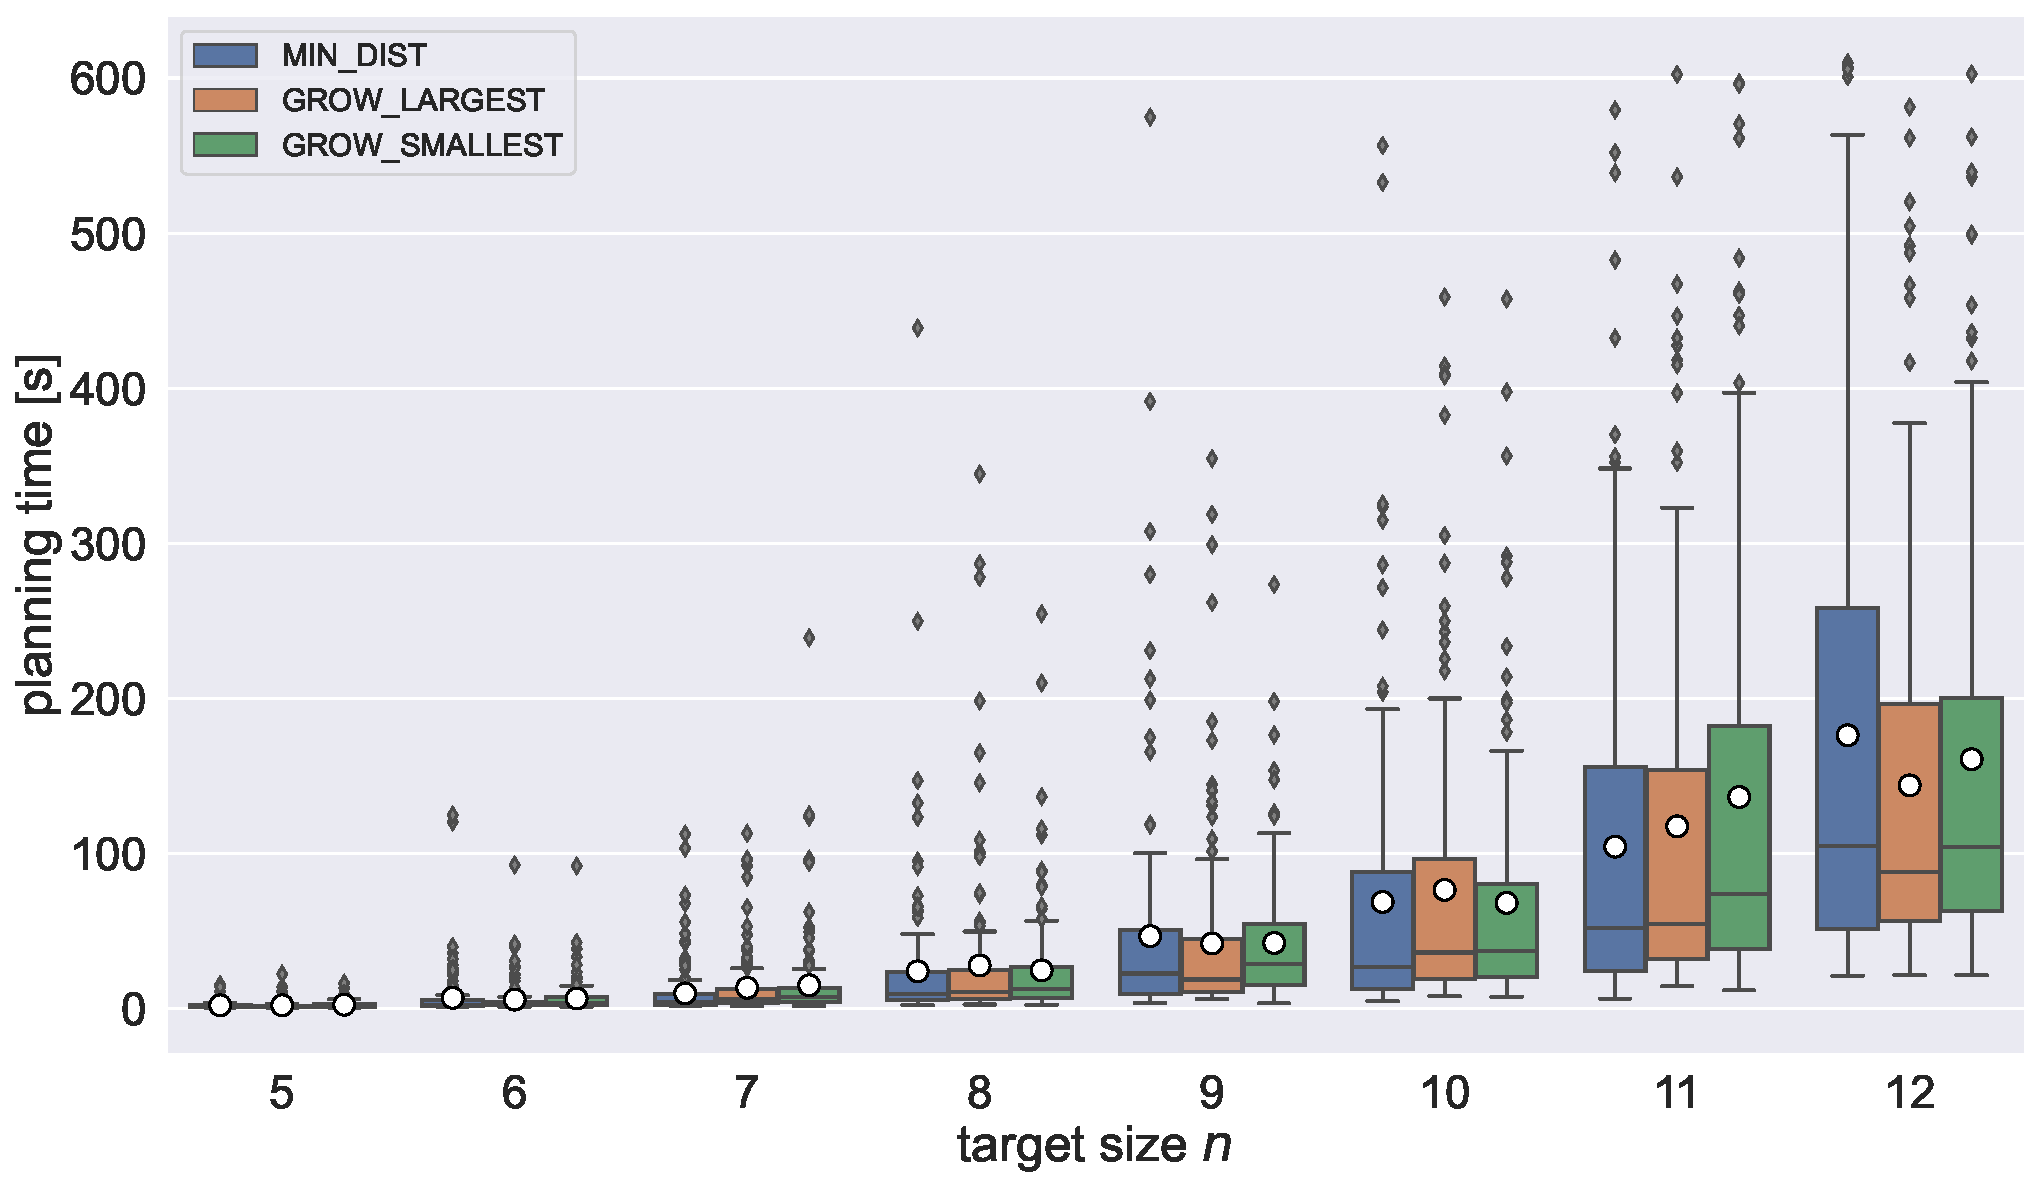
\includegraphics[width=0.9\textwidth]{figures/plots/AFN_time.pdf}
		\caption{Planning time in seconds. Only plans that did not time out are shown.}
		\label{fig:AFN_time}
	\end{subfigure}

	\begin{subfigure}[b]{\textwidth}
		\centering
		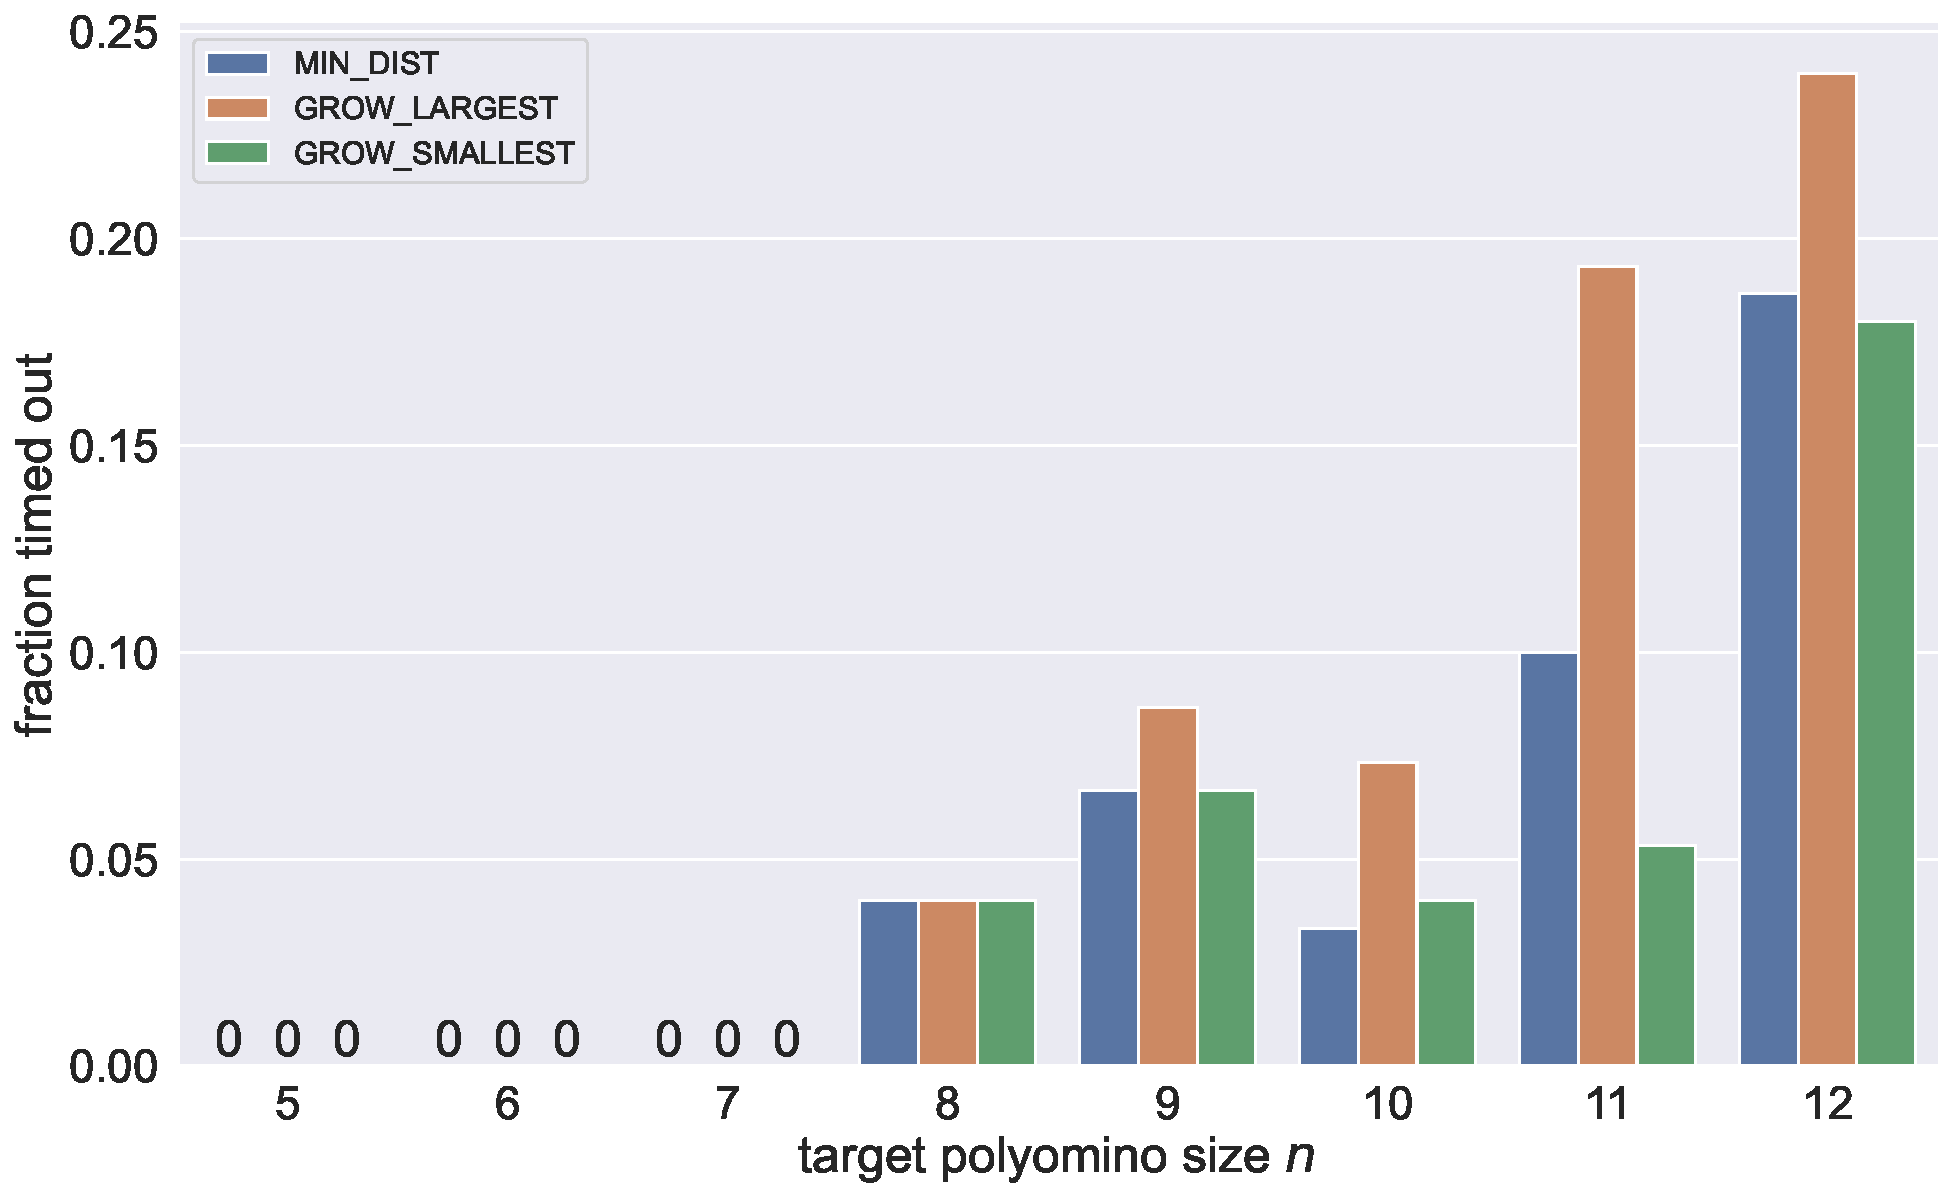
\includegraphics[width=0.9\textwidth]{figures/plots/AFN_timeout.pdf}
		\caption{Fraction of plans that timed out.}
		\label{fig:AFN_timeout}
	\end{subfigure}
	\caption[Planning time and fraction of timeouts for increasing target size]{Planning time and fraction of timeouts for increasing target size $n$. All option sorting strategies are compared.}
	\label{fig:AFN_timestats}
\end{figure}

\autoref{fig:AFN_time} shows the distribution of planning time and \autoref{fig:AFN_timeout} the fraction of timed out instances.
The construction of target polyominoes with sizes $5$ to $7$ can be planned in under $30$ seconds with just a few outliers exceeding this time.
Note the none of these instances timed out.

For target sizes above $7$ timeout failures first appear with roughly $5\%$ for $n = 8$ increasing to $20\%$ for $n=12$.
The planning time for $n = 12$ increases to $150$ seconds on average with a median of $100$ seconds.
With increasing $n$ a wider spread of planning time can be observed.
Outliers can reach planning times close to the timeout of $600$ seconds.

In terms of planning time the option sorting strategies make no noticeable difference.
For the fraction of timeouts growing the largest component often exceeds the other two strategies, clearly visible for $n=11$, where grow largest is at $20\%$ and the others under $10\%$ of plans timed out.


\paragraph{Plan Cost}

\begin{figure}
	\centering
	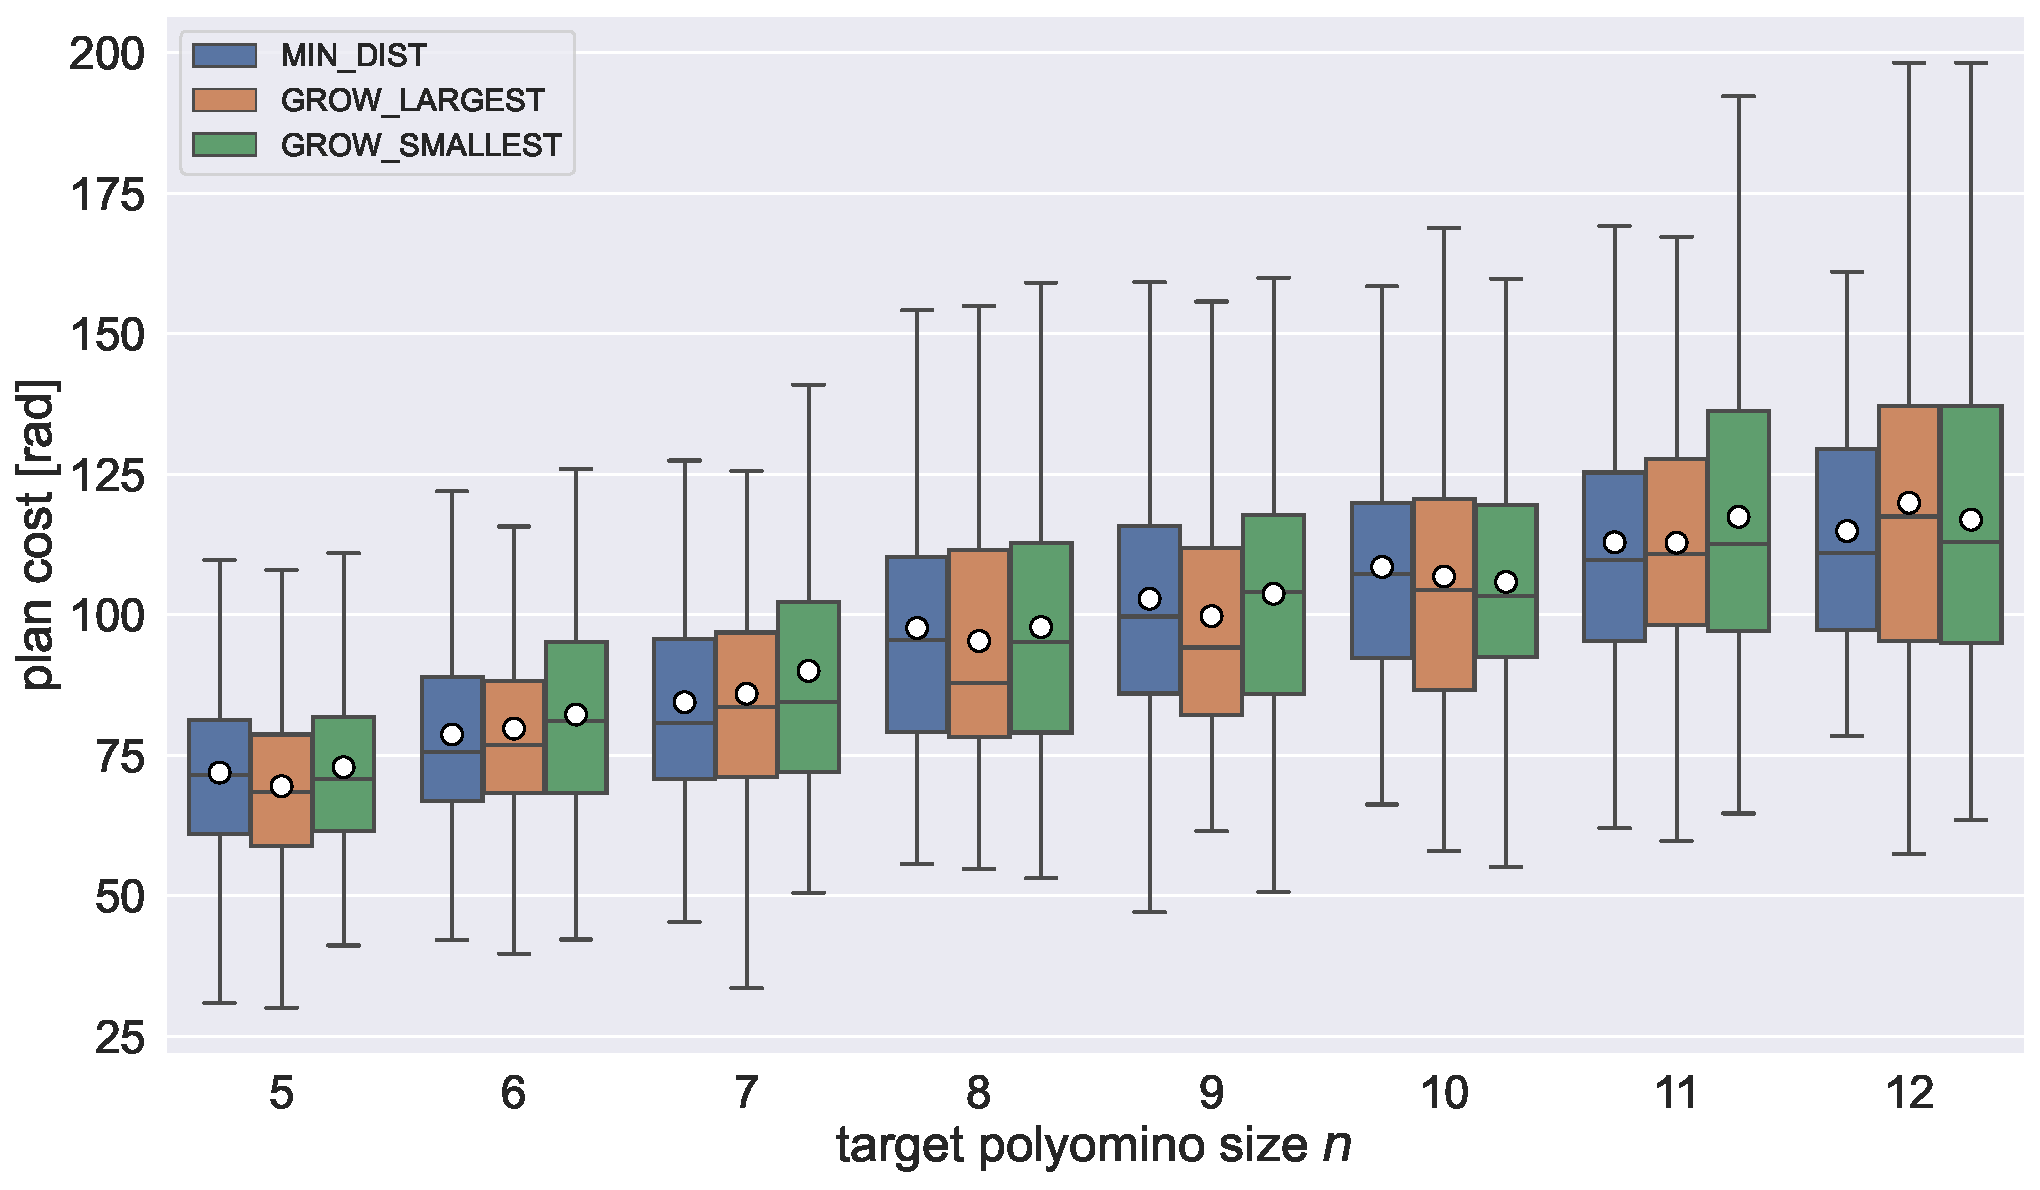
\includegraphics[width=0.9\textwidth]{figures/plots/AFN_cost.pdf}
	\caption[Plan cost for increasing size]{Plan cost in radians of successful plans for increasing target size $n$. All option sorting strategies are compared and outliers are omitted.}
	\label{fig:AFN_cost}
\end{figure}

\autoref{fig:AFN_cost} shows the rotational cost of plans that successfully assembled the target.
The cost increase slightly for bigger polyominoes, but the gradient seems to be flatting out for sizes $11$ and $12$.
Plan cost is generally in a range of $50$ to $150$ radians, which is the equivalent of $8$ to $24$ full longitude rotations of the magnetic field.
The different option sorting strategies do not impact the cost of a plan.

\paragraph{Planning Attributes}

\begin{figure}
	\centering
	\begin{subfigure}[b]{\textwidth}
		\centering
		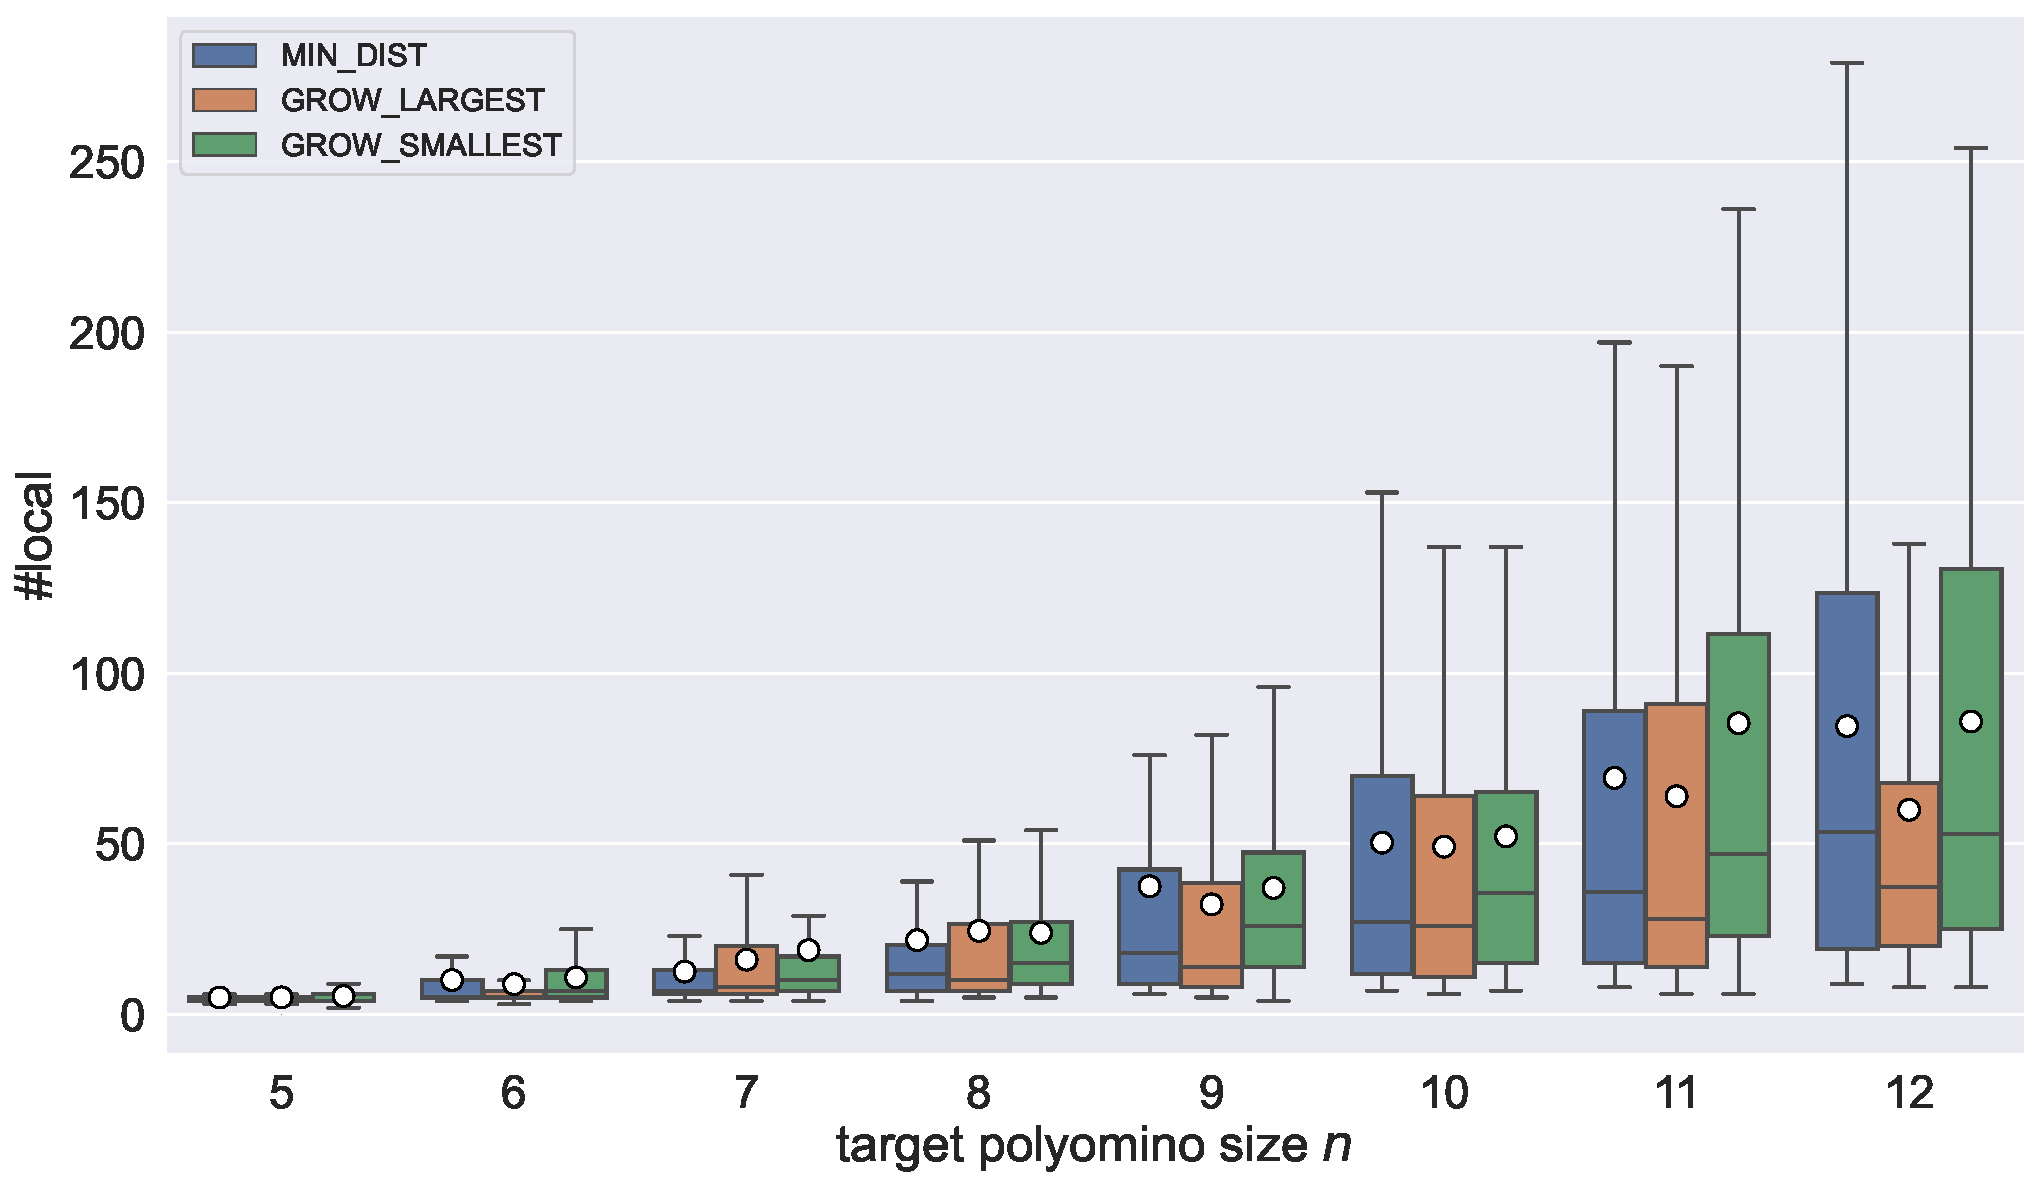
\includegraphics[width=0.9\textwidth]{figures/plots/AFN_nlocal.pdf}
		\caption{Number of simulated local plans.}
		\label{fig:AFN_nlocal}
	\end{subfigure}
	
	\begin{subfigure}[b]{\textwidth}
		\centering
		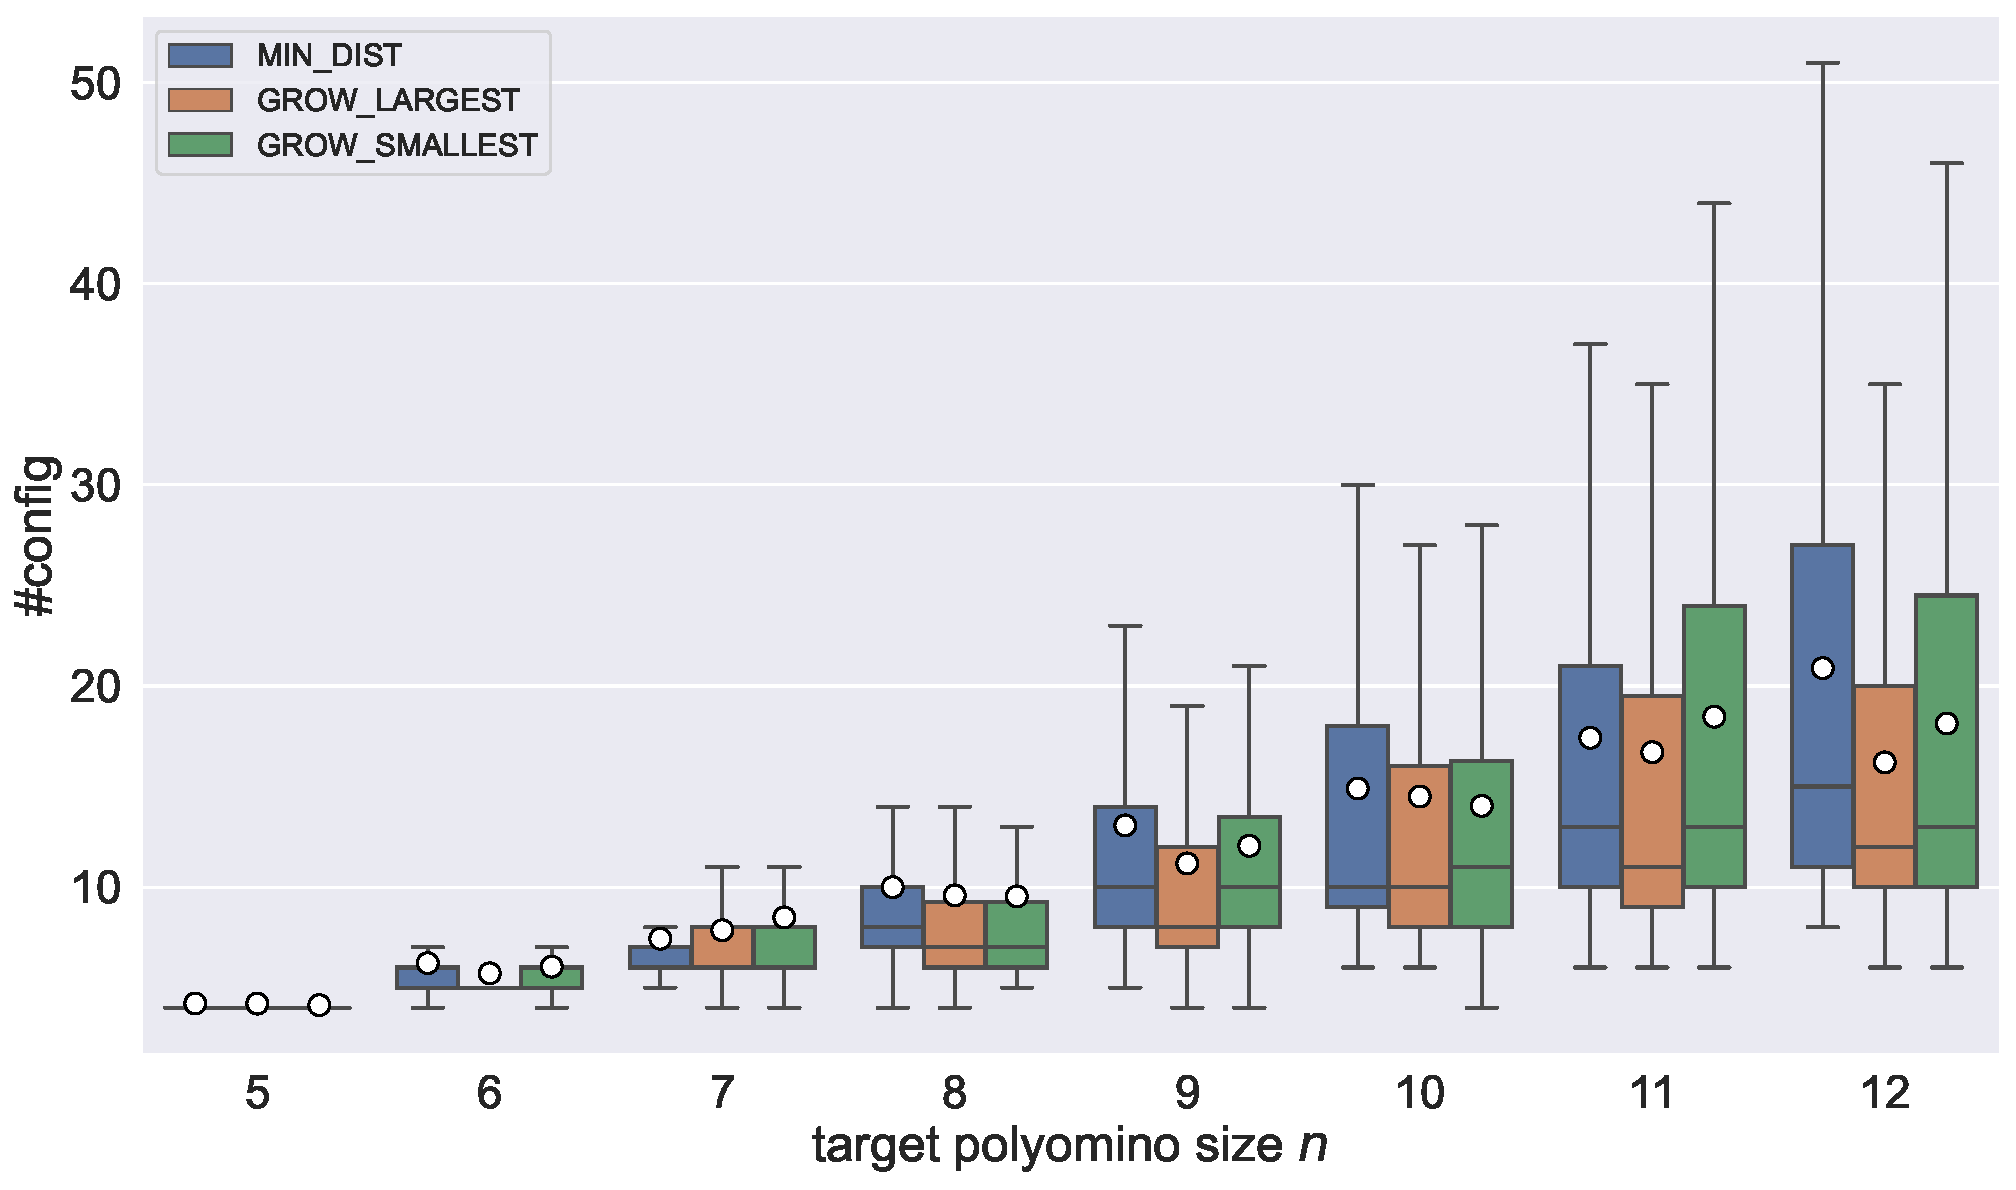
\includegraphics[width=0.9\textwidth]{figures/plots/AFN_nconfig.pdf}
		\caption{Number of explored configurations.}
		\label{fig:AFN_nconfig}
	\end{subfigure}
	\caption[Number of simulated local plans and explored configurations for increasing target size]{Number of simulated local plans $\#\textit{local}$ and explored configurations $\#\textit{config}$ for increasing target size $n$. Only plans that did not time out are shown and outliers are omitted for better readability. All option sorting strategies are compared.}
	\label{fig:AFN_planstats}
\end{figure}

\begin{figure}
	\centering
	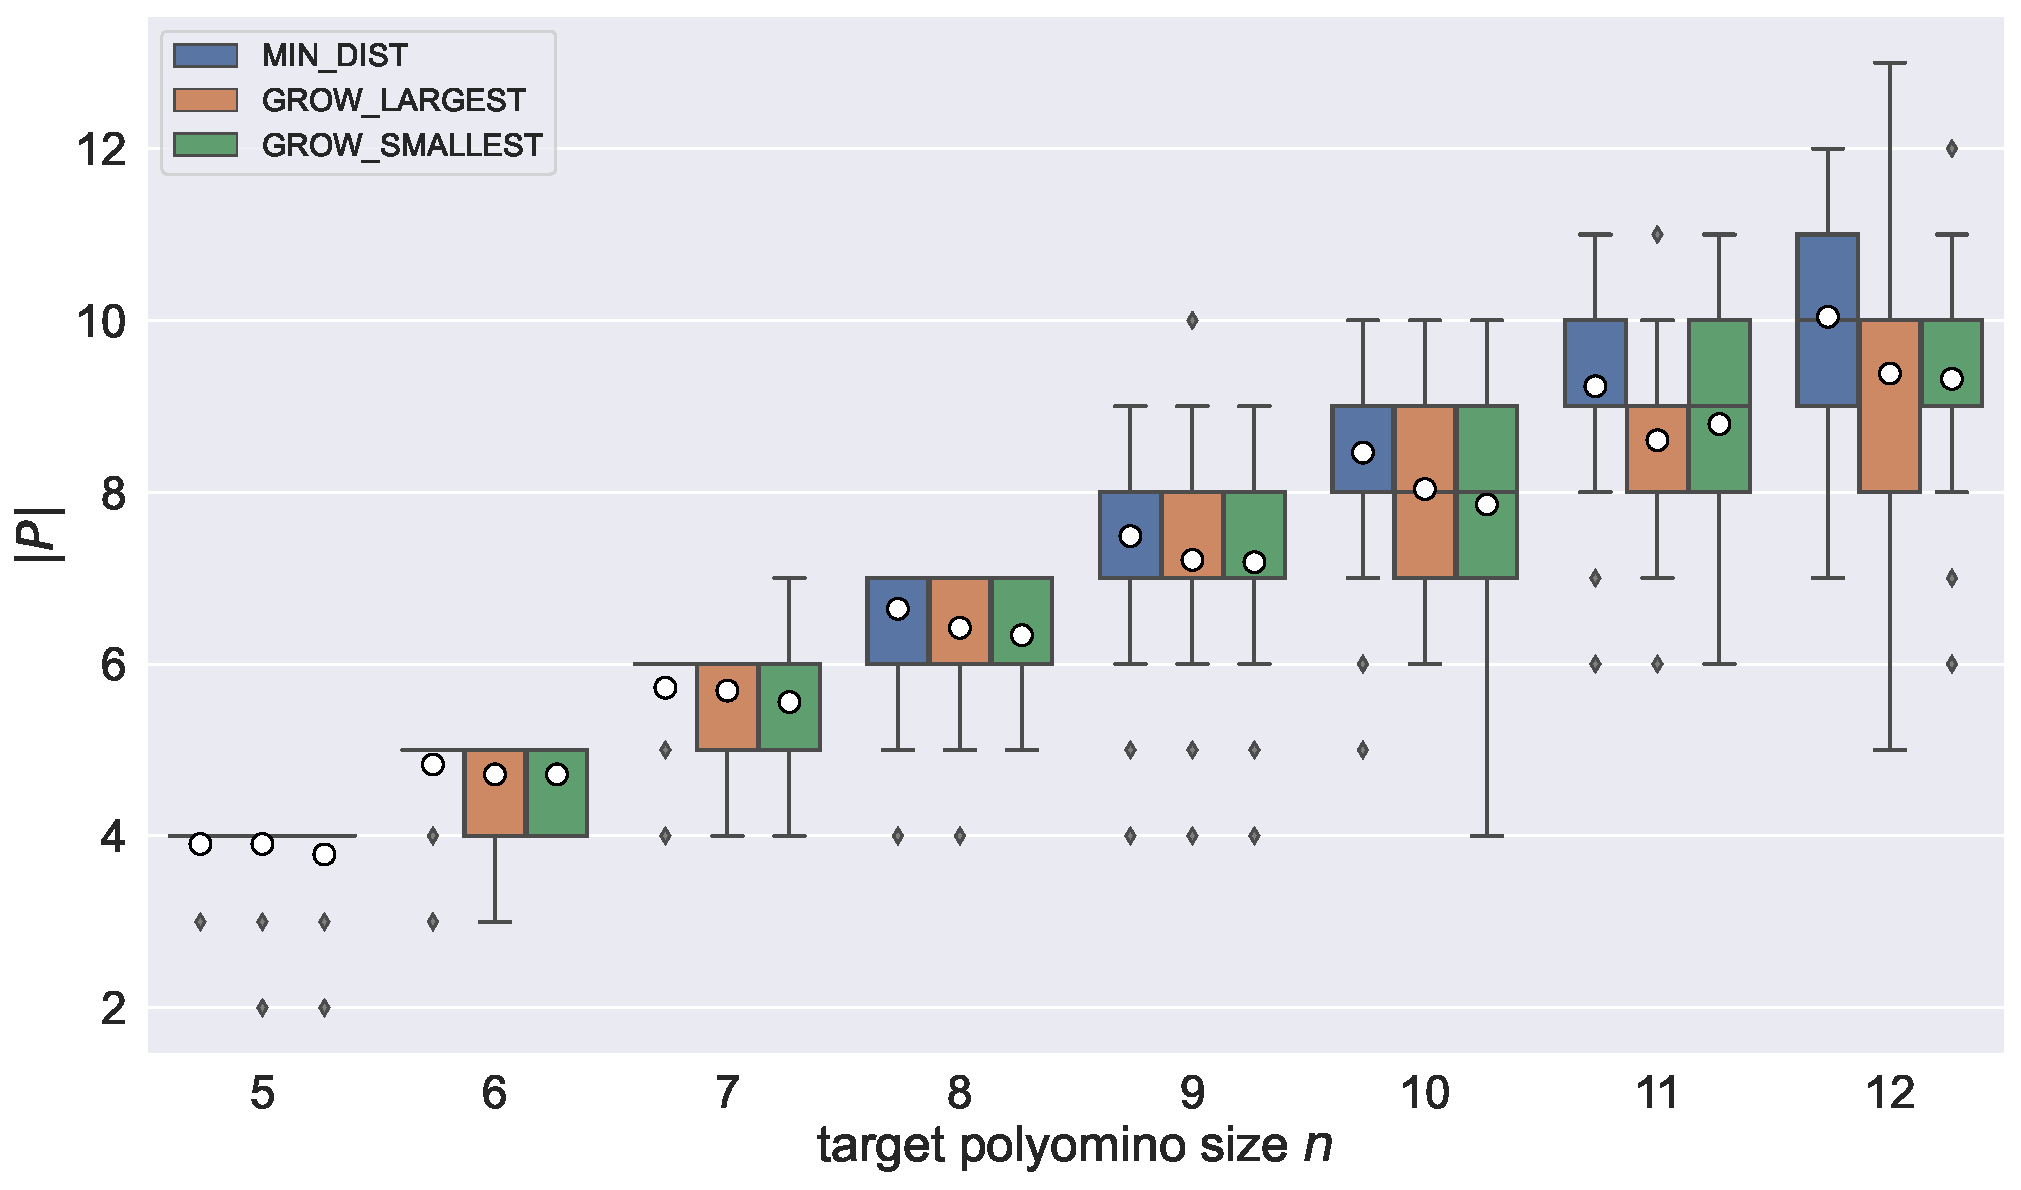
\includegraphics[width=0.9\textwidth]{figures/plots/AFN_ltg.pdf}
	\caption[Local plans in plan stack for increasing target size]{Local plans in plan stack $|P|$ for increasing target size $n$. Only successful plans are shown and all option sorting strategies are compared.}
	\label{fig:AFN_ltg}
\end{figure}


We analyze the number of simulated local plan $\#\textit{local}$ and the number of explored configuration $\#\textit{config}$ in \autoref{fig:AFN_planstats}.
The number of local plans contained in the plan stack of the resulting global plan $|P|$ is evaluated in \autoref{fig:AFN_ltg}.

When a plan times out $\#\textit{local}$ and $\#\textit{config}$ only portray how many local plan and configurations can be explored within the timeout.
Numbers can reach values up to $\#\textit{local} = 1200$ and $\#\textit{config} = 300$.
Timed out instances are omitted in the plots of \autoref{fig:AFN_planstats}.

$\#\textit{local}$ increases for bigger target polyominoes.
On average the realistic best case of $n-1$ local plans (\autoref{sec:global_complex}) is exceeded.
For $n=8$ there are $25$, for $n=10$ about $50$ and for $n=12$ roughly $75$ local plans simulated on average.
For all $n$ the majority of instances are below the average.
Outliers can reach up to $250$ local plans.

$\#\textit{config}$ behaves similarly.
The averages exceed the realistic best case of $n$, for example $\#\textit{config} = 16$ with $n=12$.
In this example the global planner encountered at least $4$ dead ends during planning.
The small numbers of $\#\textit{config}$ show that our depth first search approach is able to assemble polyominoes by only exploring a small portion of the whole configuration space.

For the majority of instances the number of local plans in the plan stack is at $|P| = n-1$.
Layer skipping can be observed frequently whenever $|P| < n-1$.
Surprisingly, instances with $|P| > n-1$ can also be observed.
This should not be possible due to a TCSA graph depth of $n$.
An explanation for this is that polyominoes break during simulation and create polyomino sets, which are at the same or a lower depth than the initial set that the local planner started with.
This phenomenon becomes more frequent for $n \geq 9$.

The only noticeable difference between the option sorting strategies is that growing the largest component tends to have slightly lower numbers of $\#\textit{config}$.

%TODO-----Prove reading-------

\section{Assembly of Custom Polyominoes}
\label{sec:AFTS}

\begin{figure}
	\centering
	\begin{subfigure}[b]{\textwidth}
		\centering
		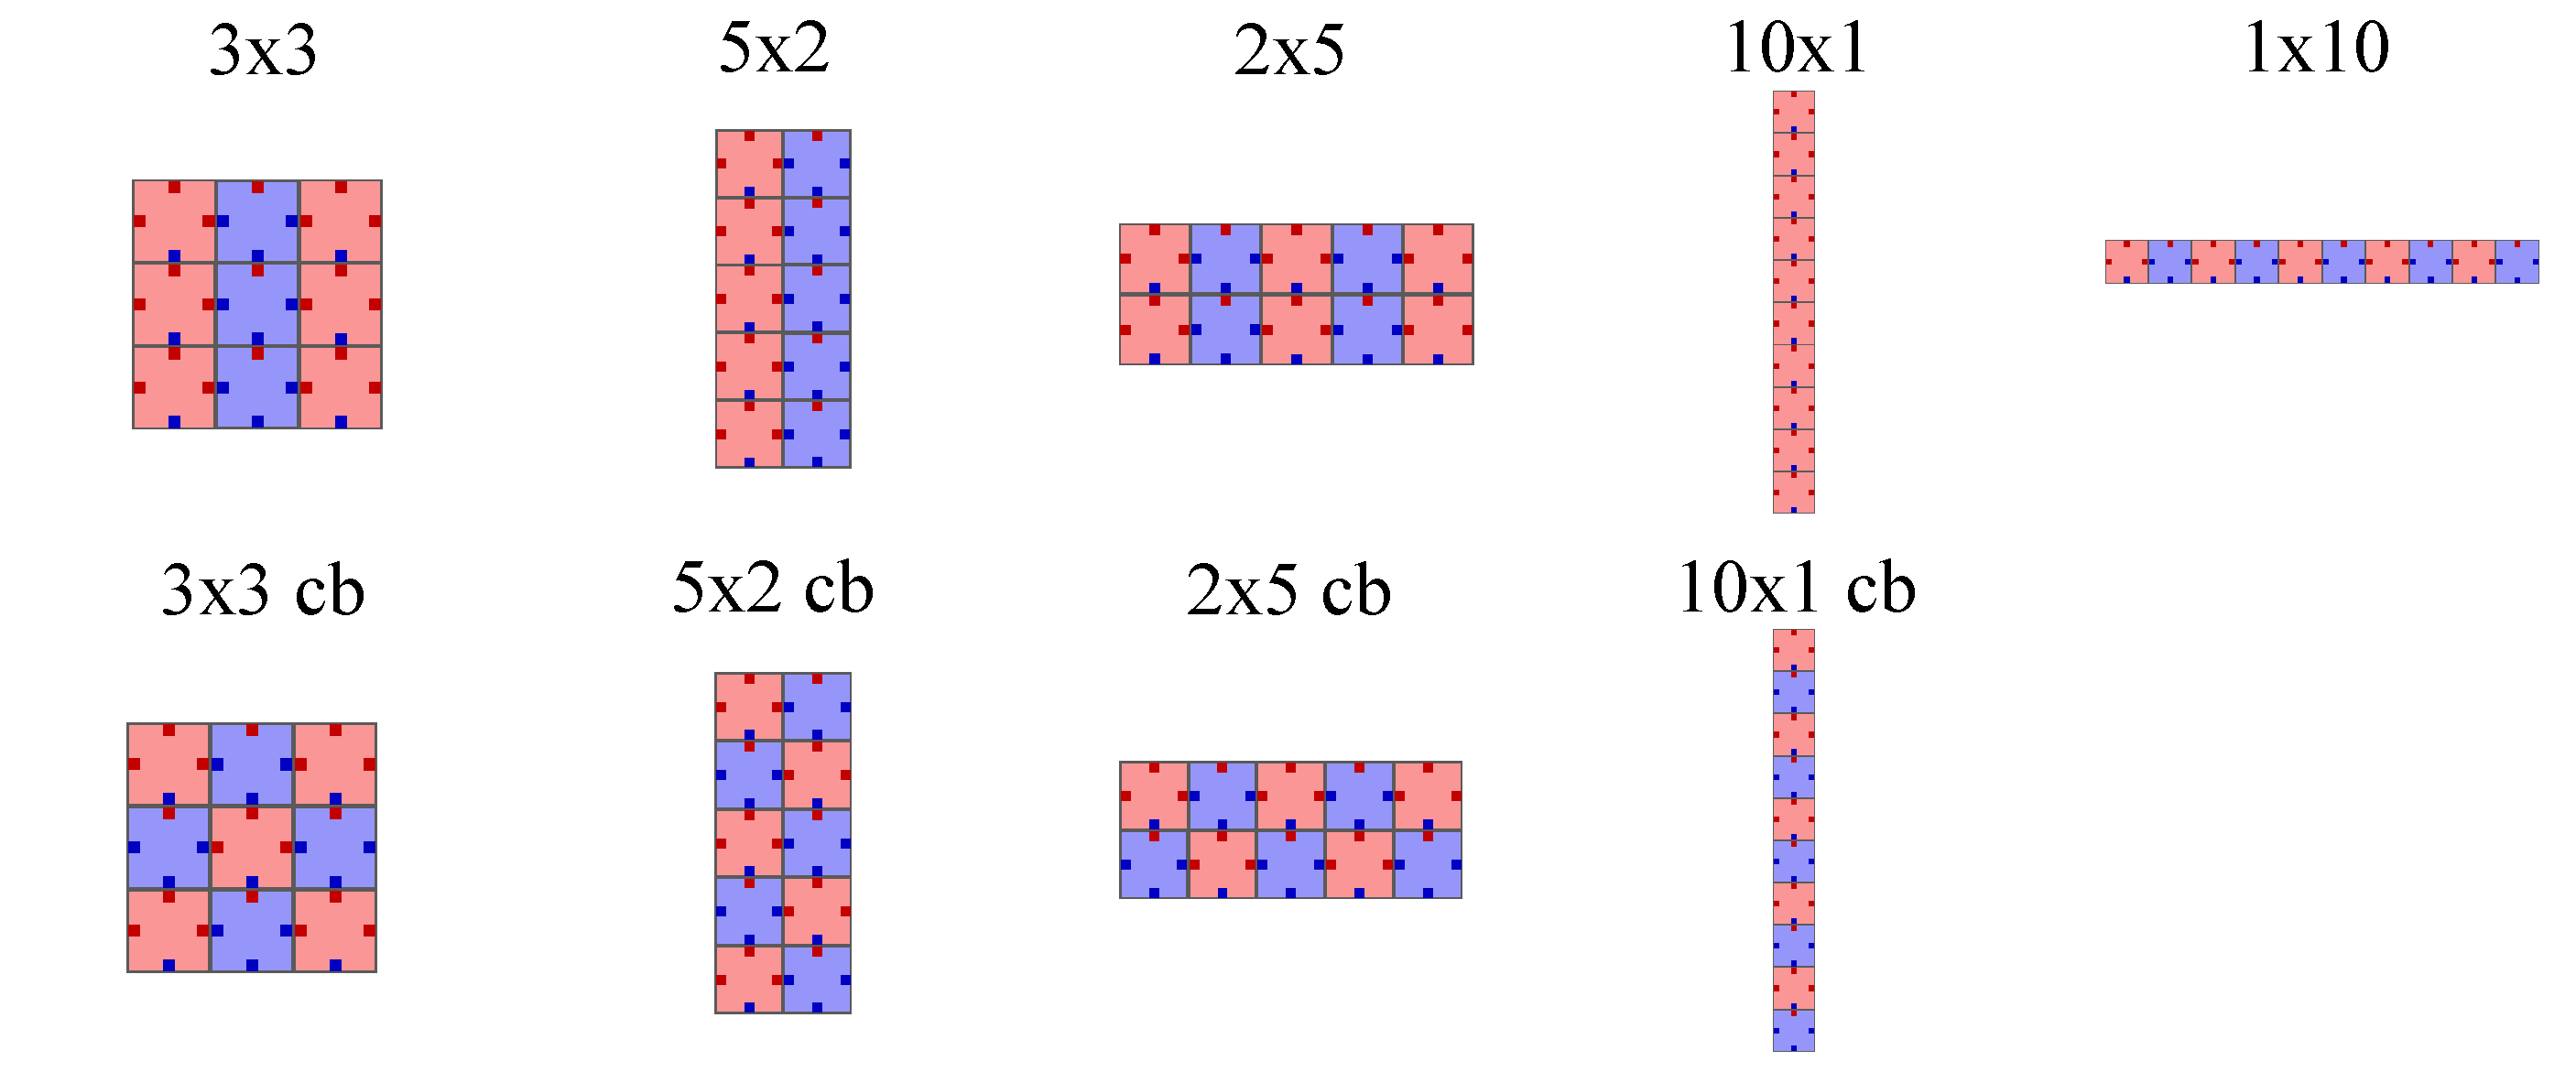
\includegraphics[width=0.8\textwidth]{figures/AFTS_cb_shapes.pdf}
		\caption{Rectangular polyominoes evaluated in \autoref{sec:w/h_pattern}. The checkerboard pattern is labeled with ``cb''. \hfill}
		\label{fig:AFTS_cb_shapes}
	\end{subfigure}
	\begin{subfigure}[b]{\textwidth}
		\centering
		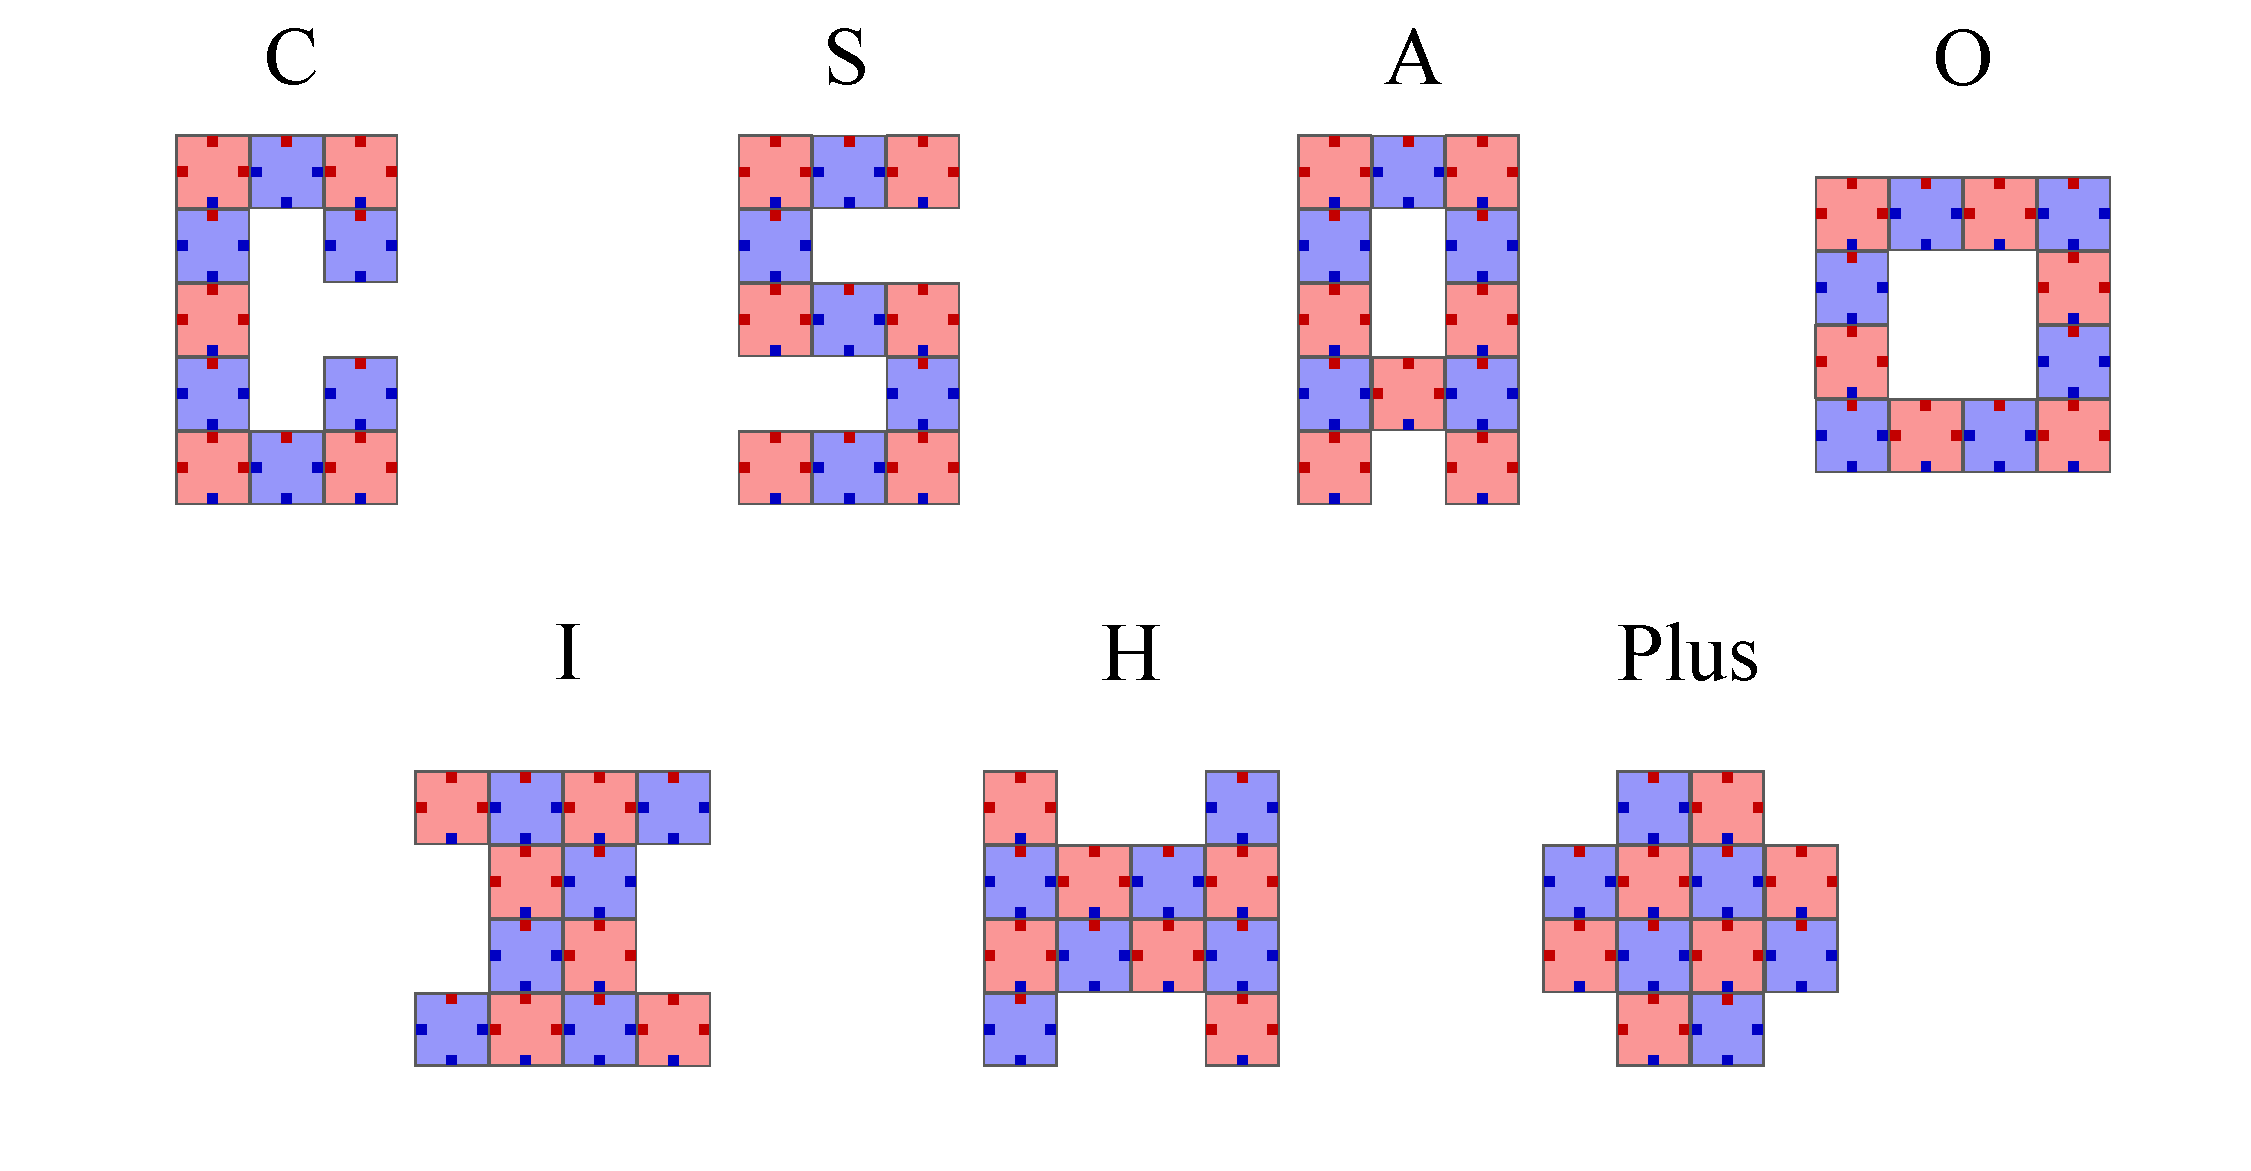
\includegraphics[width=0.7\textwidth]{figures/AFTS_sp_shapes.pdf}
		\caption{Special polyomino shapes evaluated in \autoref{sec:special_poly}.}
		\label{fig:AFTS_sp_shapes}
	\end{subfigure}
	\caption[List of manually designed polyominoes for experimenting]{List of manually designed polyominoes for experimenting.}
	\label{fig:AFTS_shapes}
\end{figure}

%TODO show number of tcsa nodes for all shapes

In this experiment manually designed polyominoes are assembled from multiple randomly generated initial configurations.
$100$ samples were taken for each custom polyomino with a workspace size of $50 r_C \times 50 r_C$.

In \autoref{sec:w/h_pattern} we focus on how rectangular polyominoes with varying width/height ratios influence planning time.
Furthermore we experiment with two patterns of red and blue for each polyomino.
The \textit{switching-column pattern} switches between red and blue cubes column vise and the \textit{checkerboard pattern} creates a checkerboard of single red and blue cubes.
A list of these polyominoes can be found in \autoref{fig:AFTS_cb_shapes}.

In \autoref{sec:special_poly} the assembly of special polyomino shapes, that are listed in \autoref{fig:AFTS_sp_shapes}, is examined. 
The polyominoes ``C'', ``S'', ``A'' and ``O'' contain caves and/or holes of different sizes, but are thin shapes with fewer connections.
They more or less consist of a one cube thick line.
The polyominoes ``I'', ``H'' and ``Plus'' are thick shapes with many connections, but still contain caves or are at least not rectangular.
All these polyominoes are build with the checkerboard pattern to archive equal amounts of red and blue cubes.
The size of all polyominoes, except for ``C'', is $n=12$.
 

\subsection{Width/Height and Cube Pattern}
\label{sec:w/h_pattern}

\begin{figure}
	\centering
	\begin{subfigure}[b]{\textwidth}
		\centering
		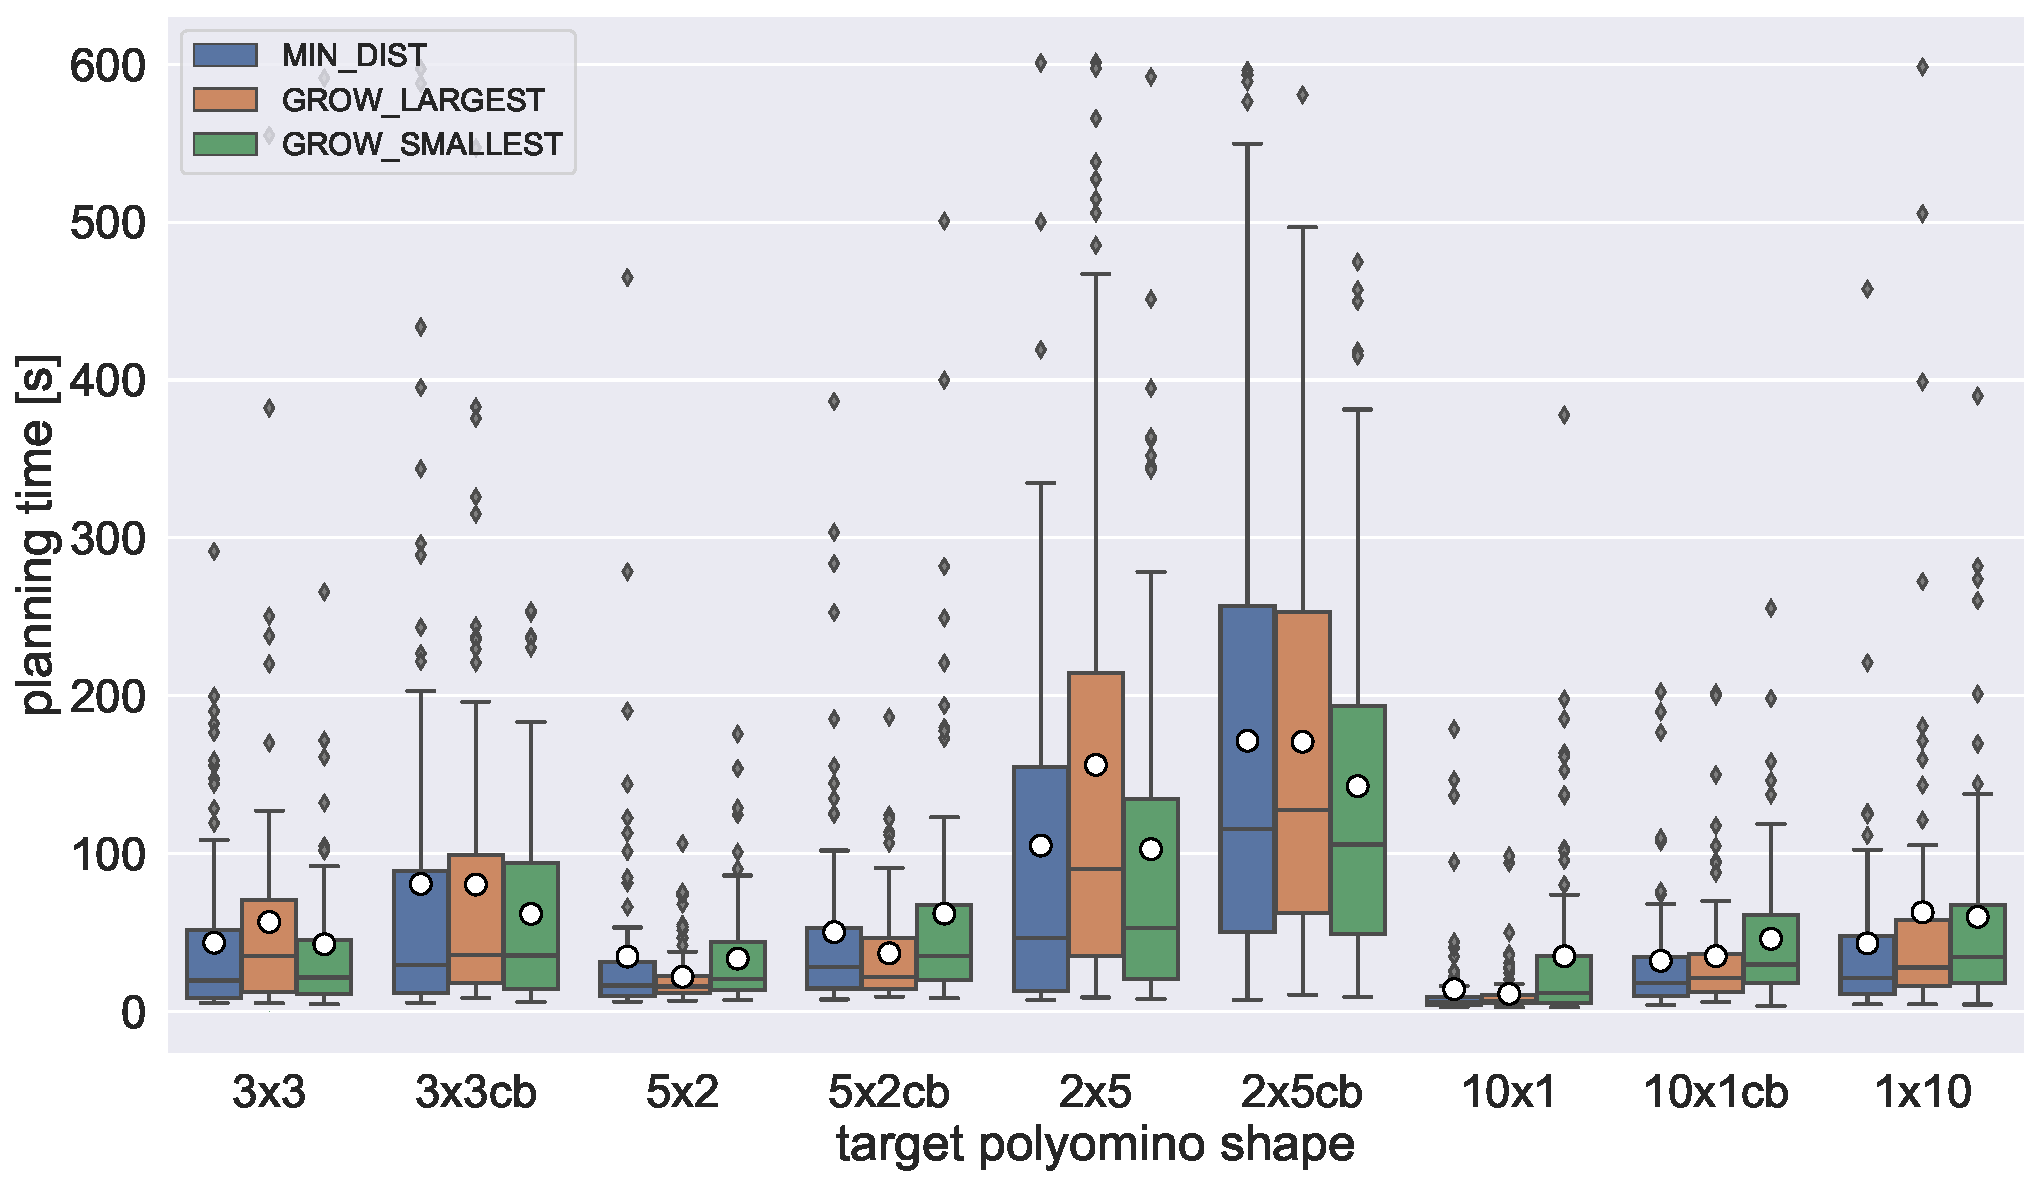
\includegraphics[width=0.9\textwidth]{figures/plots/AFTS_cb_time.pdf}
		\caption{Planning time in seconds. Only plans that did not time out are shown.}
		\label{fig:AFTS_cb_time}
	\end{subfigure}
	
	\begin{subfigure}[b]{\textwidth}
		\centering
		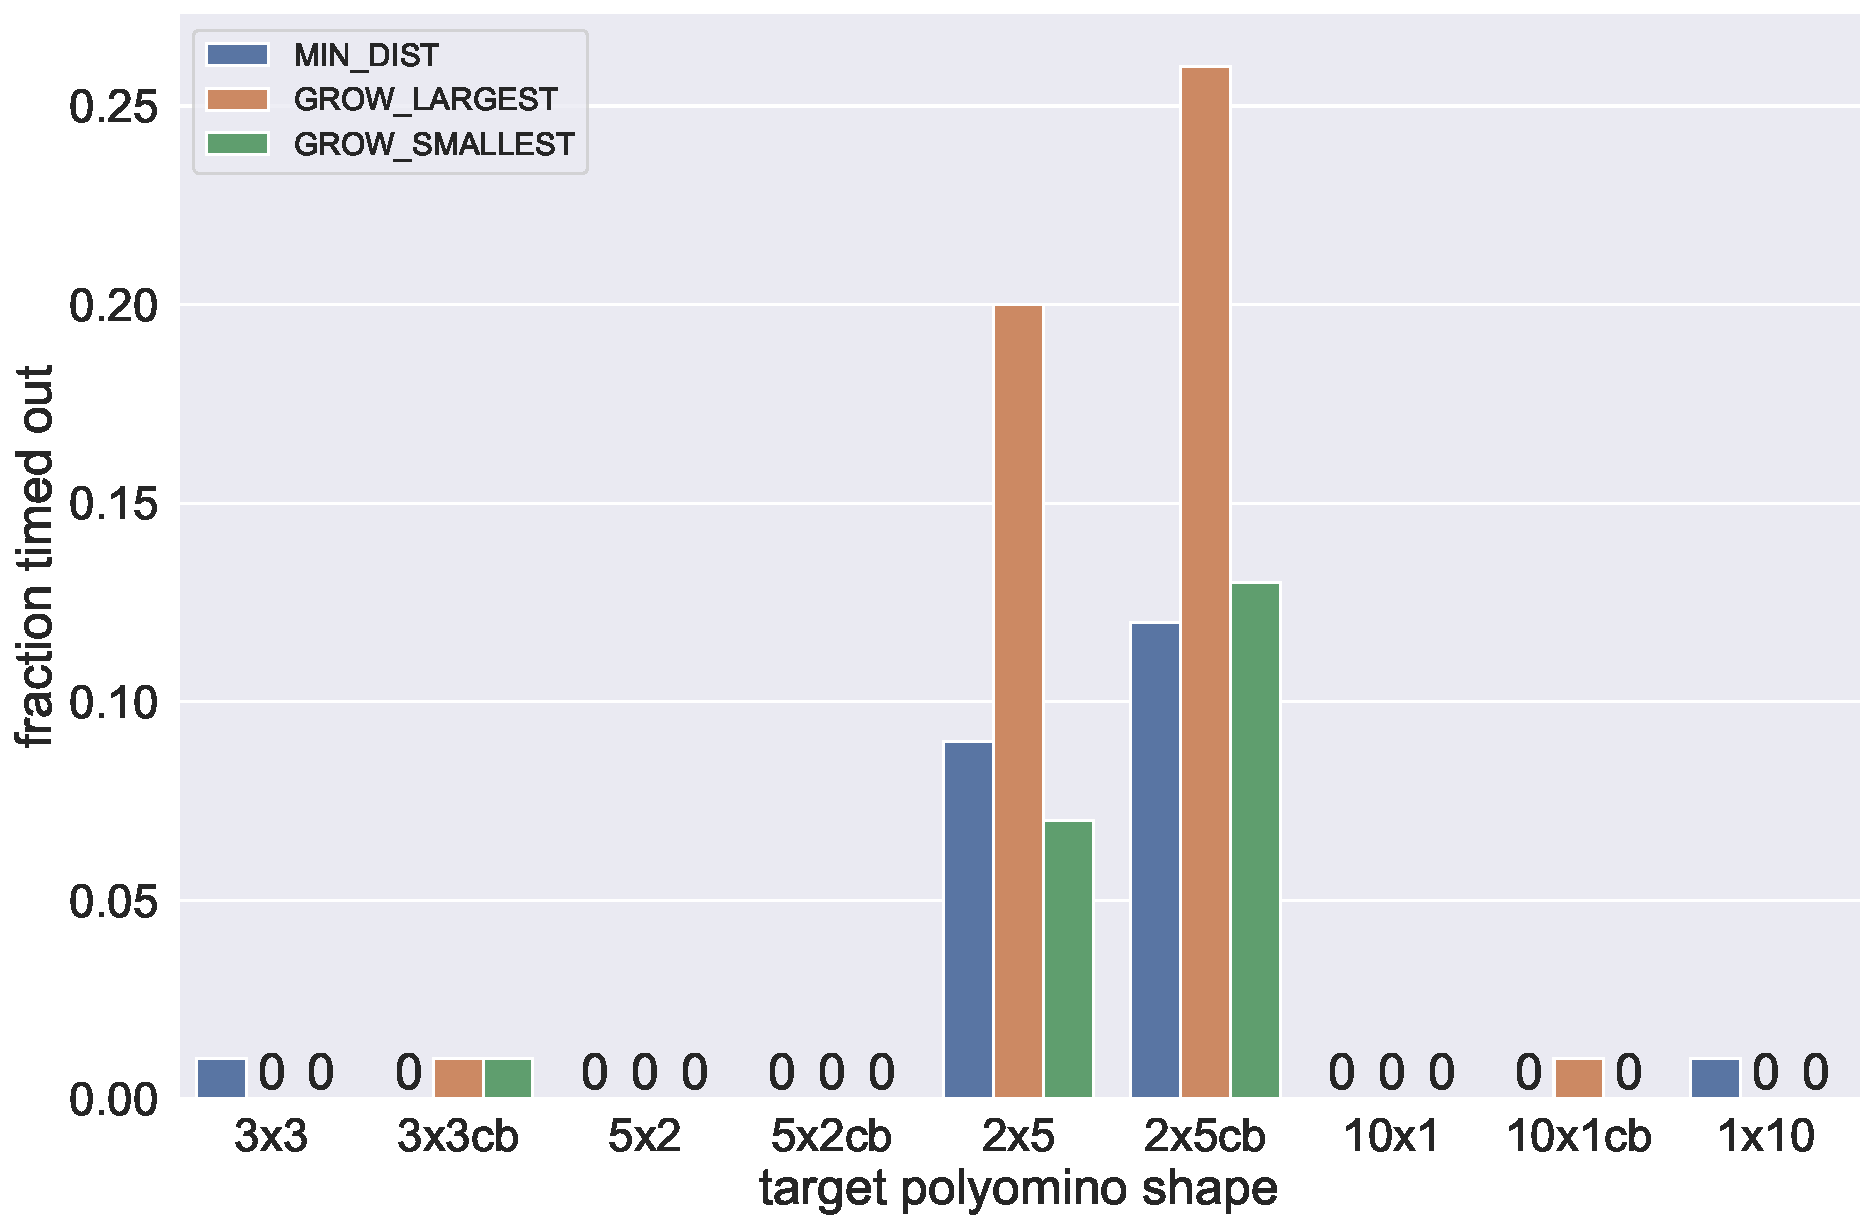
\includegraphics[width=0.9\textwidth]{figures/plots/AFTS_cb_timeout.pdf}
		\caption{Fraction of plans that timed out.}
		\label{fig:AFTS_cb_timeout}
	\end{subfigure}
	\caption[Planning time and fraction timed out for rectangular polyominoes]{Planning time and fraction timed out for rectangular polyominoes listed in \autoref{fig:AFTS_cb_shapes}. All option sorting strategies are compared.}
	\label{fig:AFTS_cb_timestats}
\end{figure}
%TODO shows shapes under plot

When comparing the two cube pattern in \autoref{fig:AFTS_cb_time}, the checkerboard pattern performs worst for all types of rectangular polyominoes.
It is not a huge difference, but still noticeable.
For instance, the ``3x3'' polyomino is on average at $50$ seconds planning time, while the ``3x3 cb'' polyomino is at 75 seconds with a wider spread and worst outliers.

Polyomino shapes with more height than width are faster to assemble.
``10x1'' is the best followed by ``5x2'', ``3x3'' and ``2x5''.
The same order persists for the checkerboard pattern.
Surprisingly the ``1x10'' polyomino breaks out of this order.
Its planning time lays between the ``5x2'' and the ``3x3''.
The ``2x5'' performs significantly worst than all other polyominoes.
While the majority of instances for all other shapes can be solved in under $100$ seconds, the ``2x5'' exceeds this time with a spread reaching up to $600$ seconds.

For the fraction of timed out plans shown in \autoref{fig:AFTS_cb_timeout}, the ``2x5'' is the only shape with $10\%$ to $20\%$, depending on the option sorting strategy.
All other shapes experience nearly no timeouts.

\subsection{Special Polyomino Shapes}
\label{sec:special_poly}

\begin{figure}
	\centering
	\begin{subfigure}[b]{\textwidth}
		\centering
		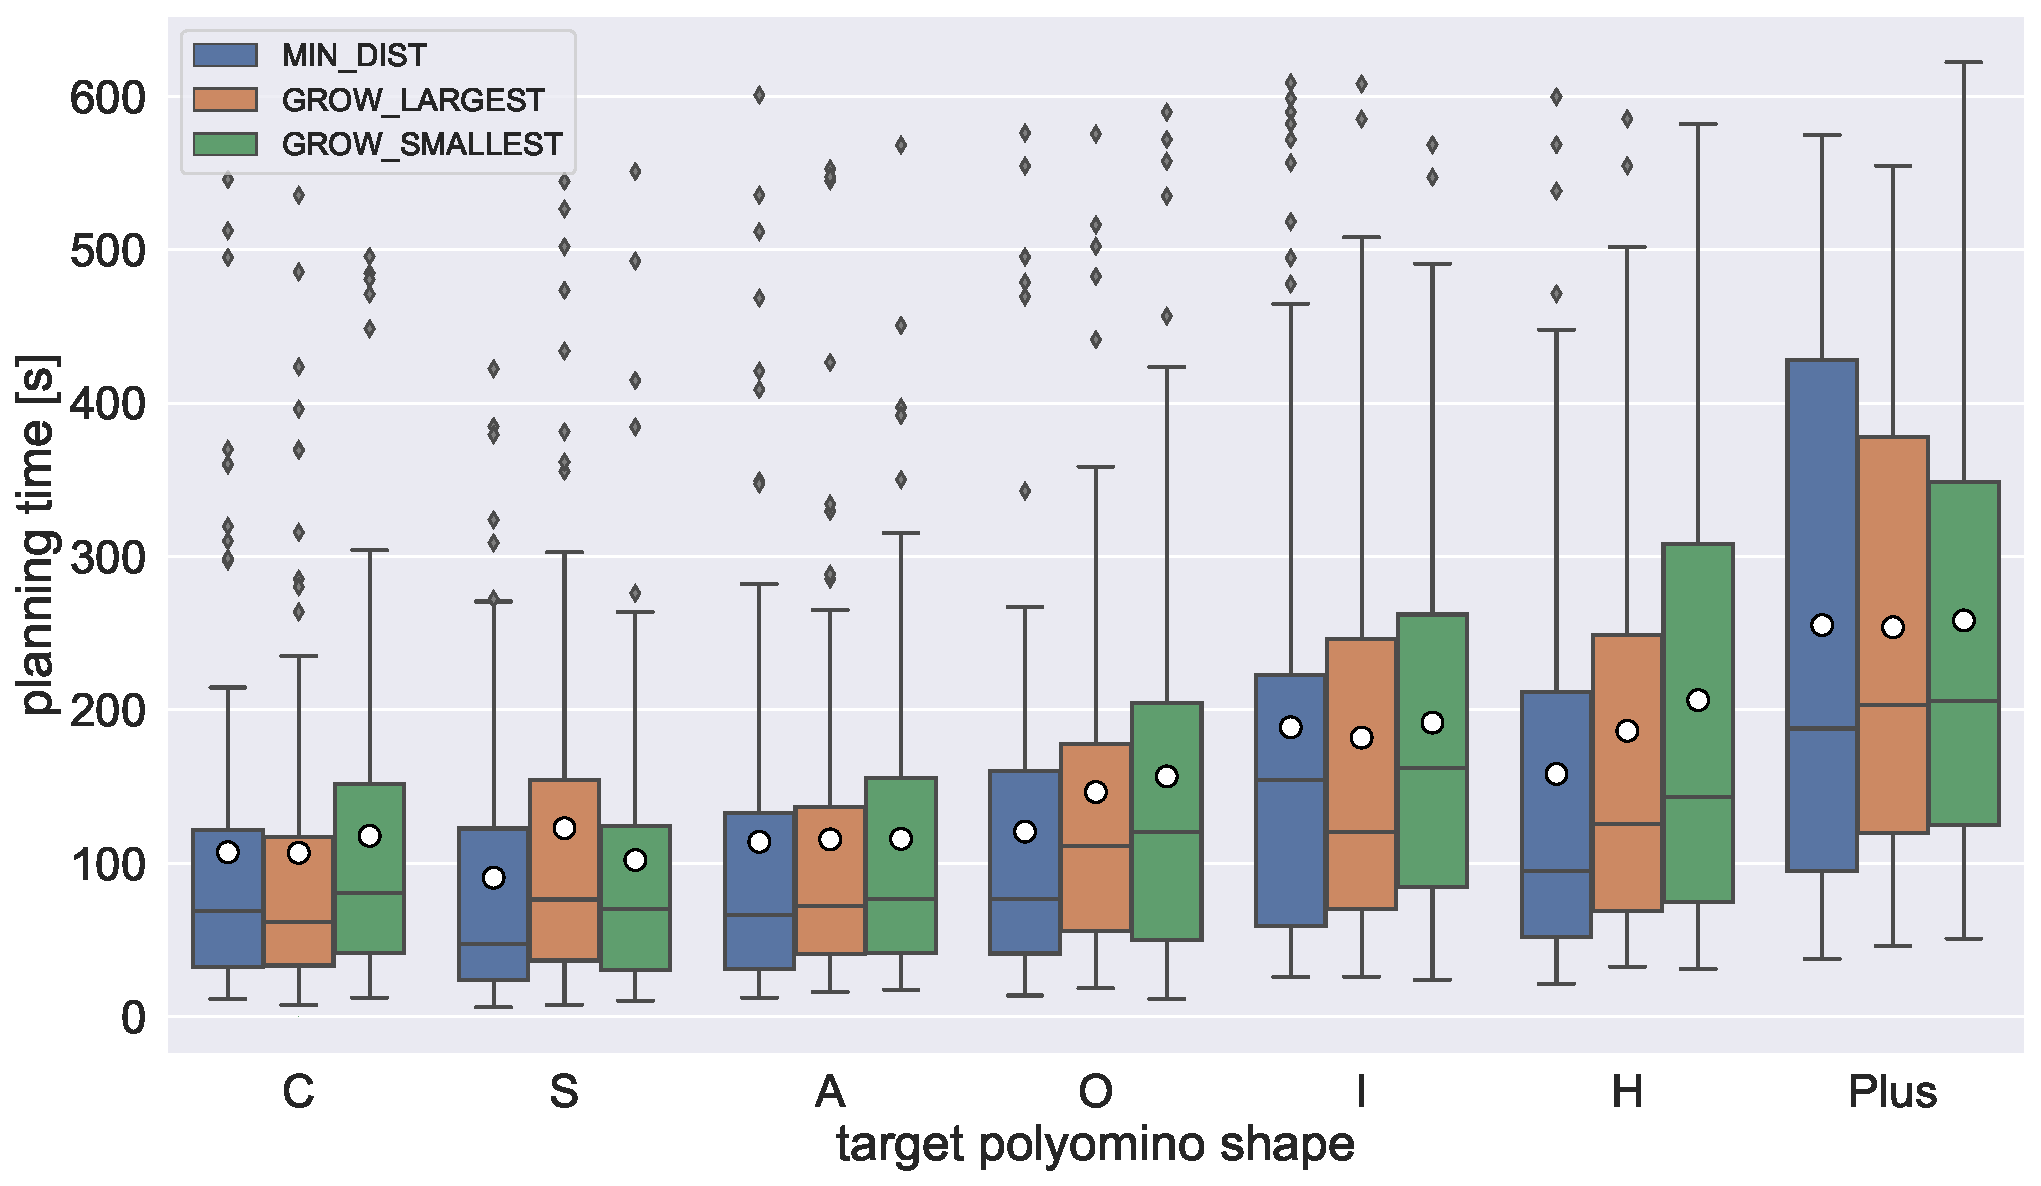
\includegraphics[width=0.9\textwidth]{figures/plots/AFTS_sp_time.pdf}
		\caption{}
		\label{fig:AFTS_sp_time}
	\end{subfigure}
	
	\begin{subfigure}[b]{\textwidth}
		\centering
		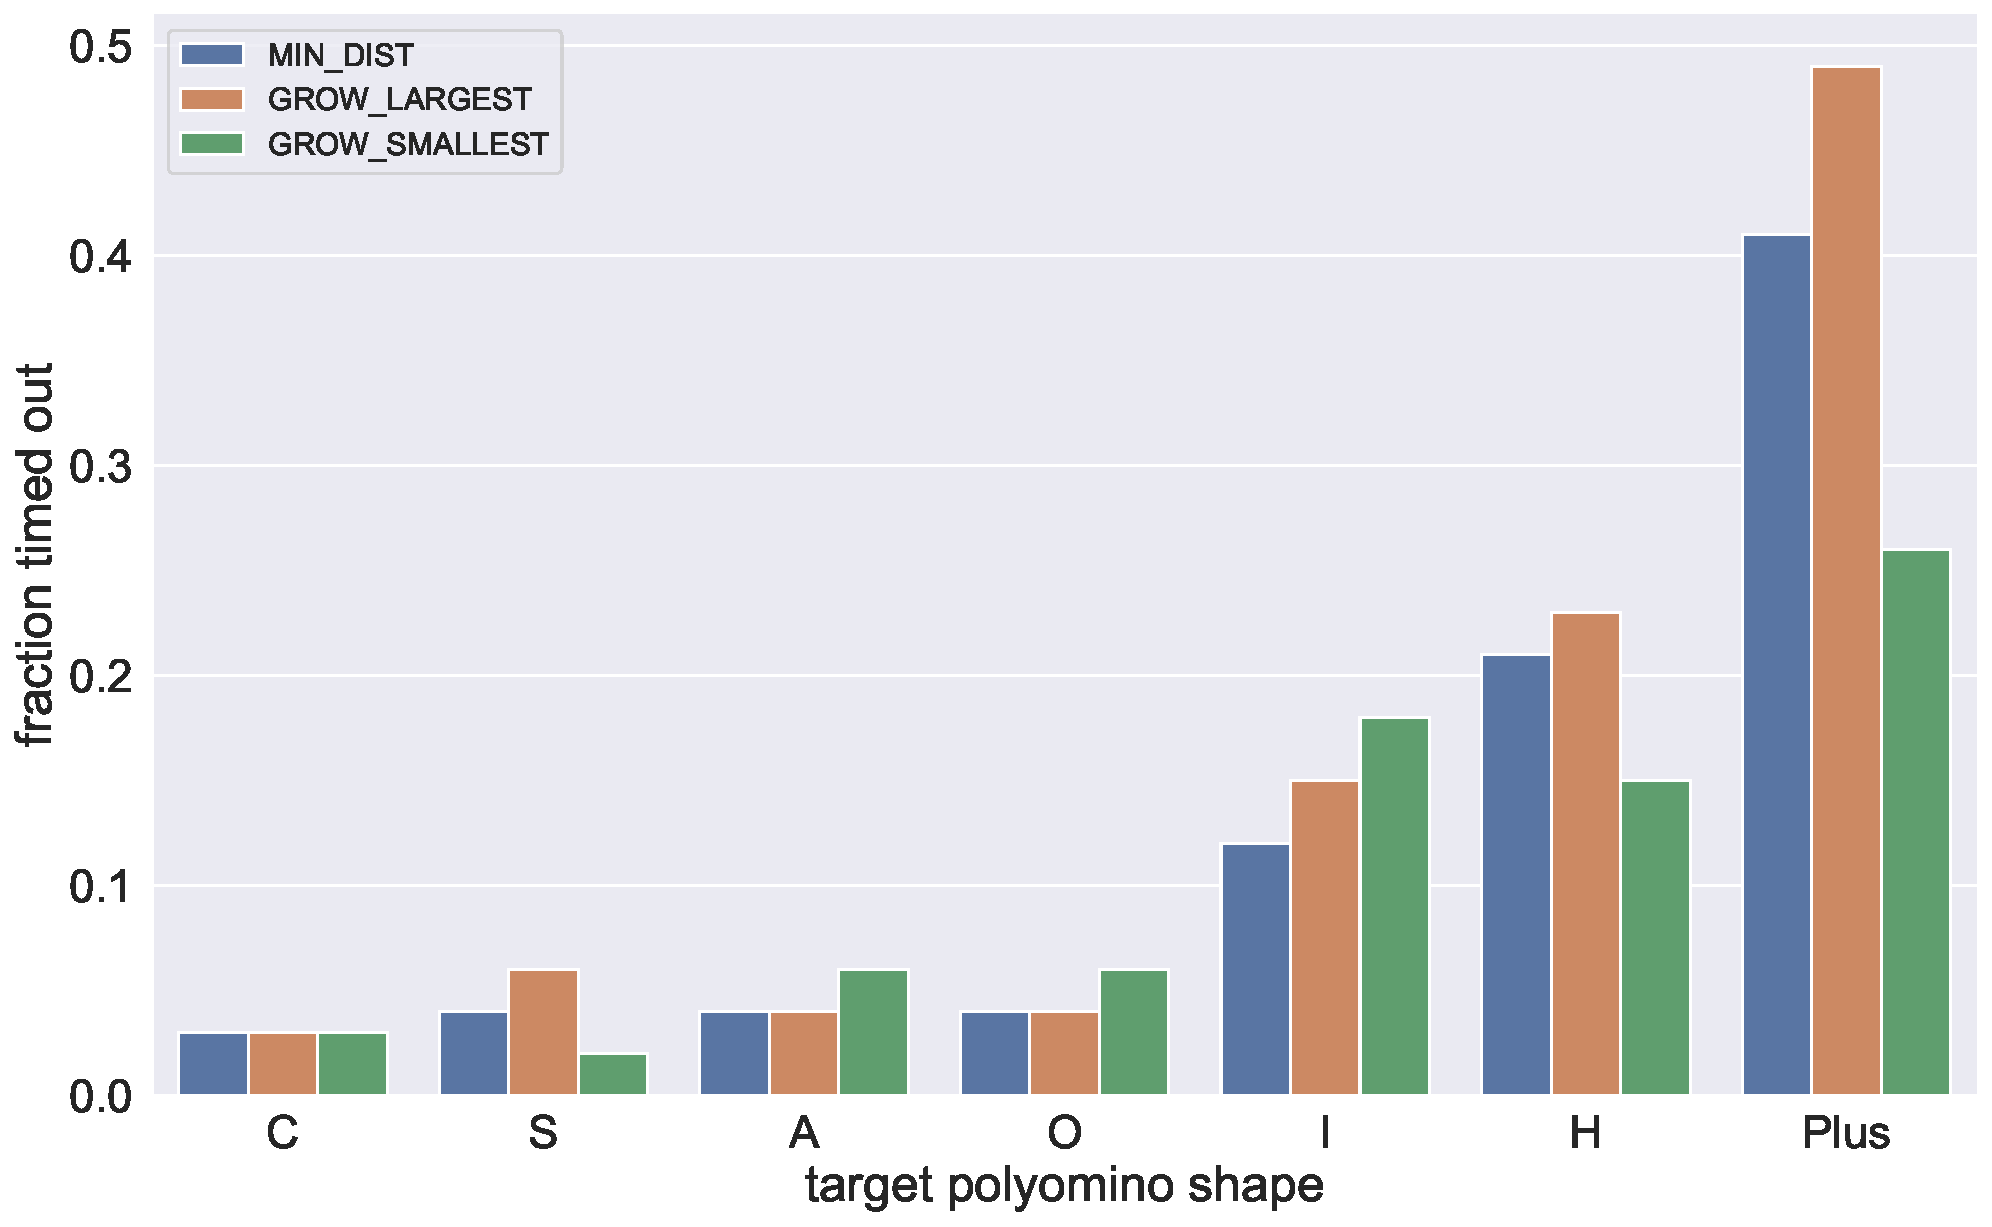
\includegraphics[width=0.9\textwidth]{figures/plots/AFTS_sp_timeout.pdf}
		\caption{}
		\label{fig:AFTS_sp_timeout}
	\end{subfigure}
	\caption[]{}
	\label{fig:AFTS_sp_timestats}
\end{figure}

Text


\section{Assembly in different Workspaces}
\label{sec:AFBS}

\begin{table}
	\centering
	\begin{tabular}{|c c|c|}
		\hline
		\multicolumn{2}{|c|}{\textbf{Workspace}} & \textbf{Width $\times$ Height}\\
		\hline
		S,& $ 1:1 $ & $35 r_C \times 35 r_C$\\
		\hline
		M,& $ 1:1 $ & $50 r_C \times 50 r_C$ \\
		\hline
		L,& $ 1:1 $ & $65 r_C \times 65 r_C$ \\
		\hline
		S,& $ 2:1 $ & $50 r_C \times 25 r_C$\\
		\hline
		M,& $ 2:1 $ & $70 r_C \times 35 r_C$ \\
		\hline
		L,& $ 2:1 $ & $90 r_C \times 45 r_C$ \\
		\hline
		S,& $ 3:1 $ & $60 r_C \times 20 r_C$\\
		\hline
		M,& $ 3:1 $ & $90 r_C \times 30 r_C$ \\
		\hline
		L,& $ 3:1 $ & $105 r_C \times 35 r_C$ \\
		\hline
	\end{tabular}
	\caption{Workspace variations with different areas and aspect ratios.}
	\label{tab:workspaces}
\end{table}

In this experiment we tested the assembly of randomly generated polyominoes of size $n=9$ with random initial configurations in various rectangular workspaces.
We choose three workspace sizes (S, M, L) in three different aspect ratios ($ 1:1 $, $ 2:1 $, $ 3:1 $) each.
All aspect ratios for one size result in roughly the same area. The workspaces with their exact widths and heights are listed in \autoref{tab:workspaces}.
A workspace with aspect ration $ 1:x $ would produce similar results to one with aspect ration $ x:1 $, since the magnetic field can be rotated freely.
The maximum width or height of a polyomino with size $9$ is $18 r_C$.
We ensured that such a polyomino could fit in all workspace variations while being able to rotate 360 degrees.
We analyze the affect of these workspace variations on planning time and rotational cost.

\paragraph{Planning Time} 

\begin{figure}
	\centering
	\begin{subfigure}[b]{\textwidth}
		\centering
		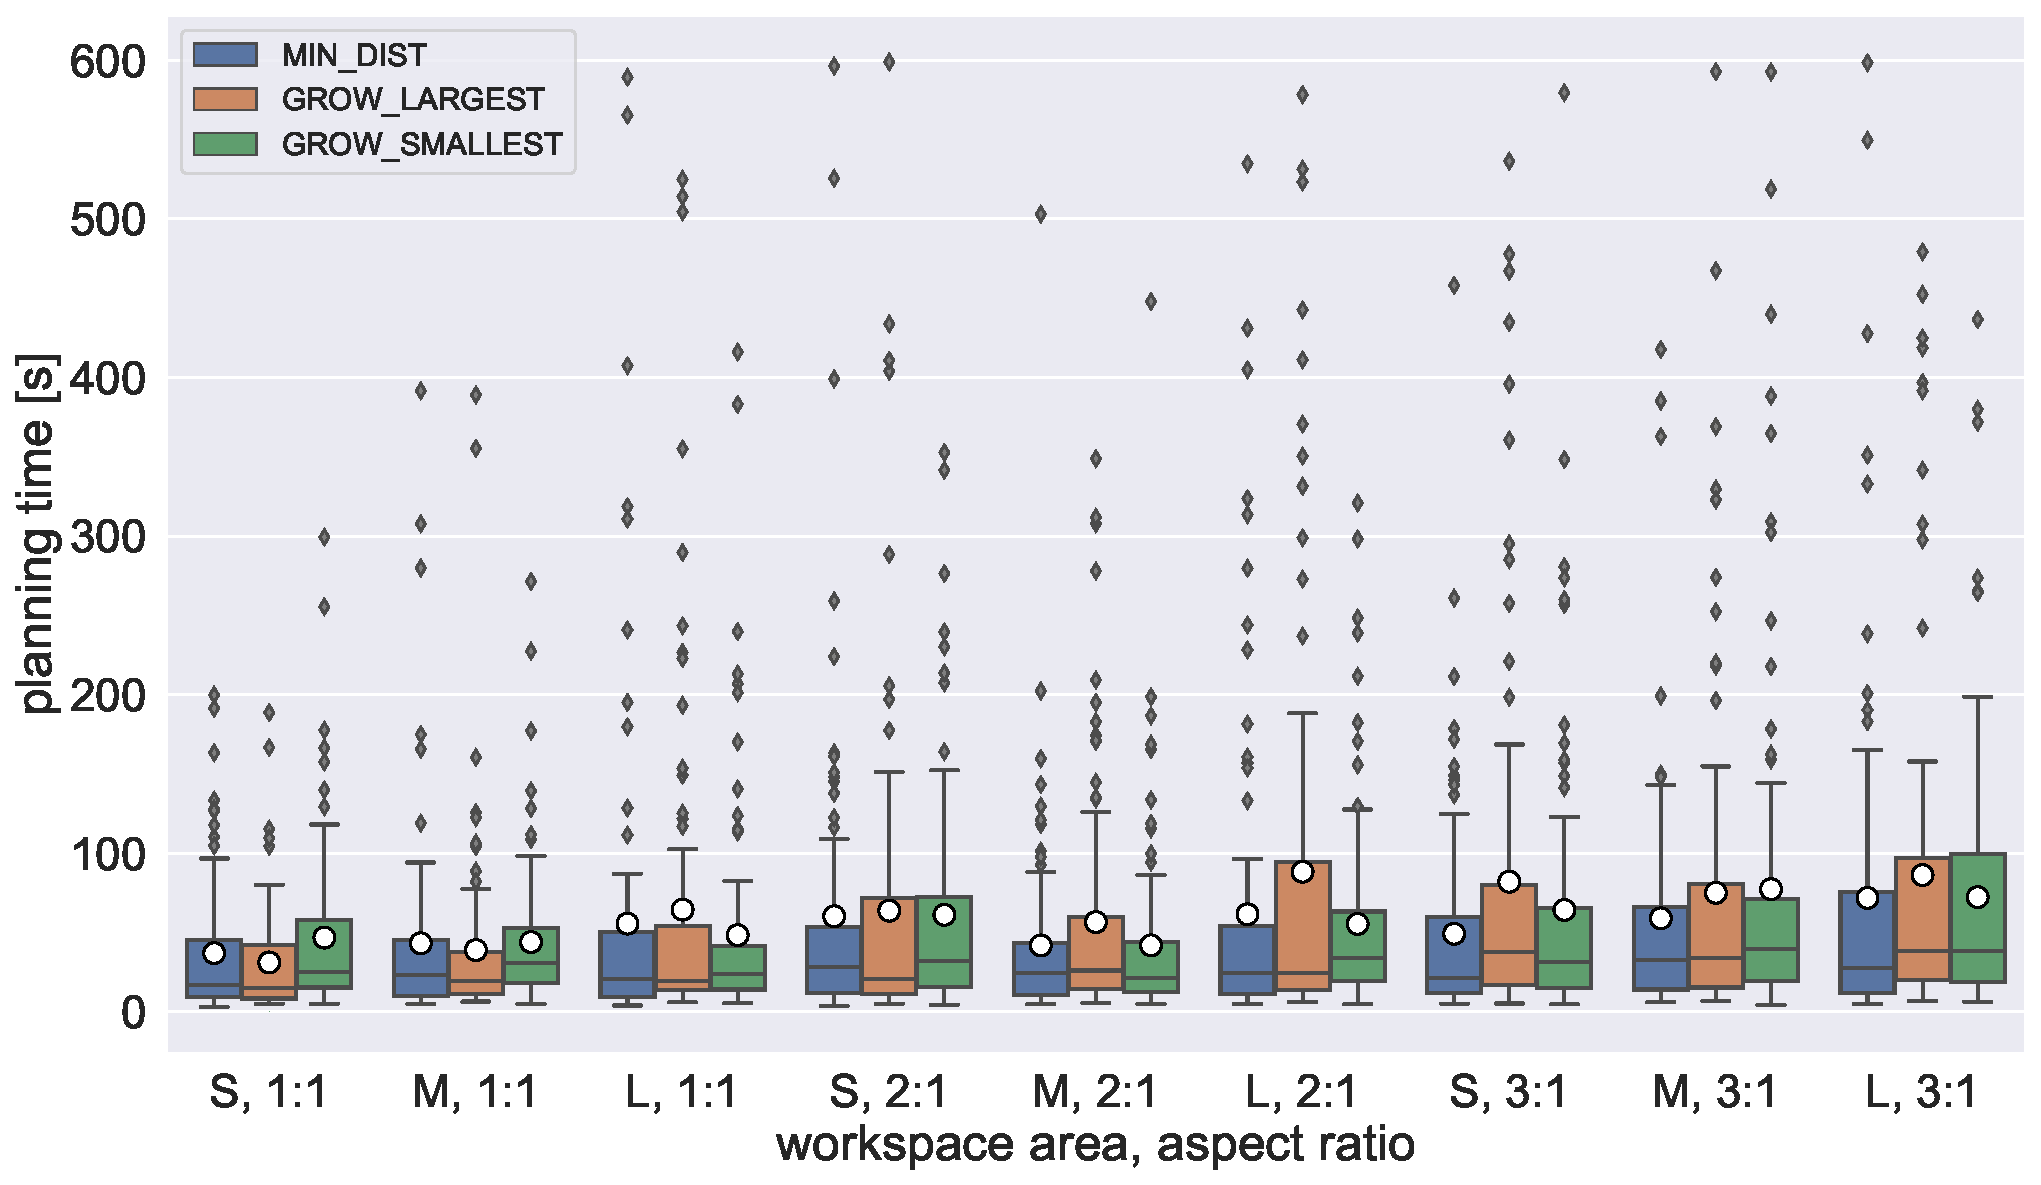
\includegraphics[width=0.9\textwidth]{figures/plots/AFBS_time.pdf}
		\caption{Planning time in seconds. Only plans that did not time out are shown.}
		\label{fig:AFBS_time}
	\end{subfigure}
	
	\begin{subfigure}[b]{\textwidth}
		\centering
		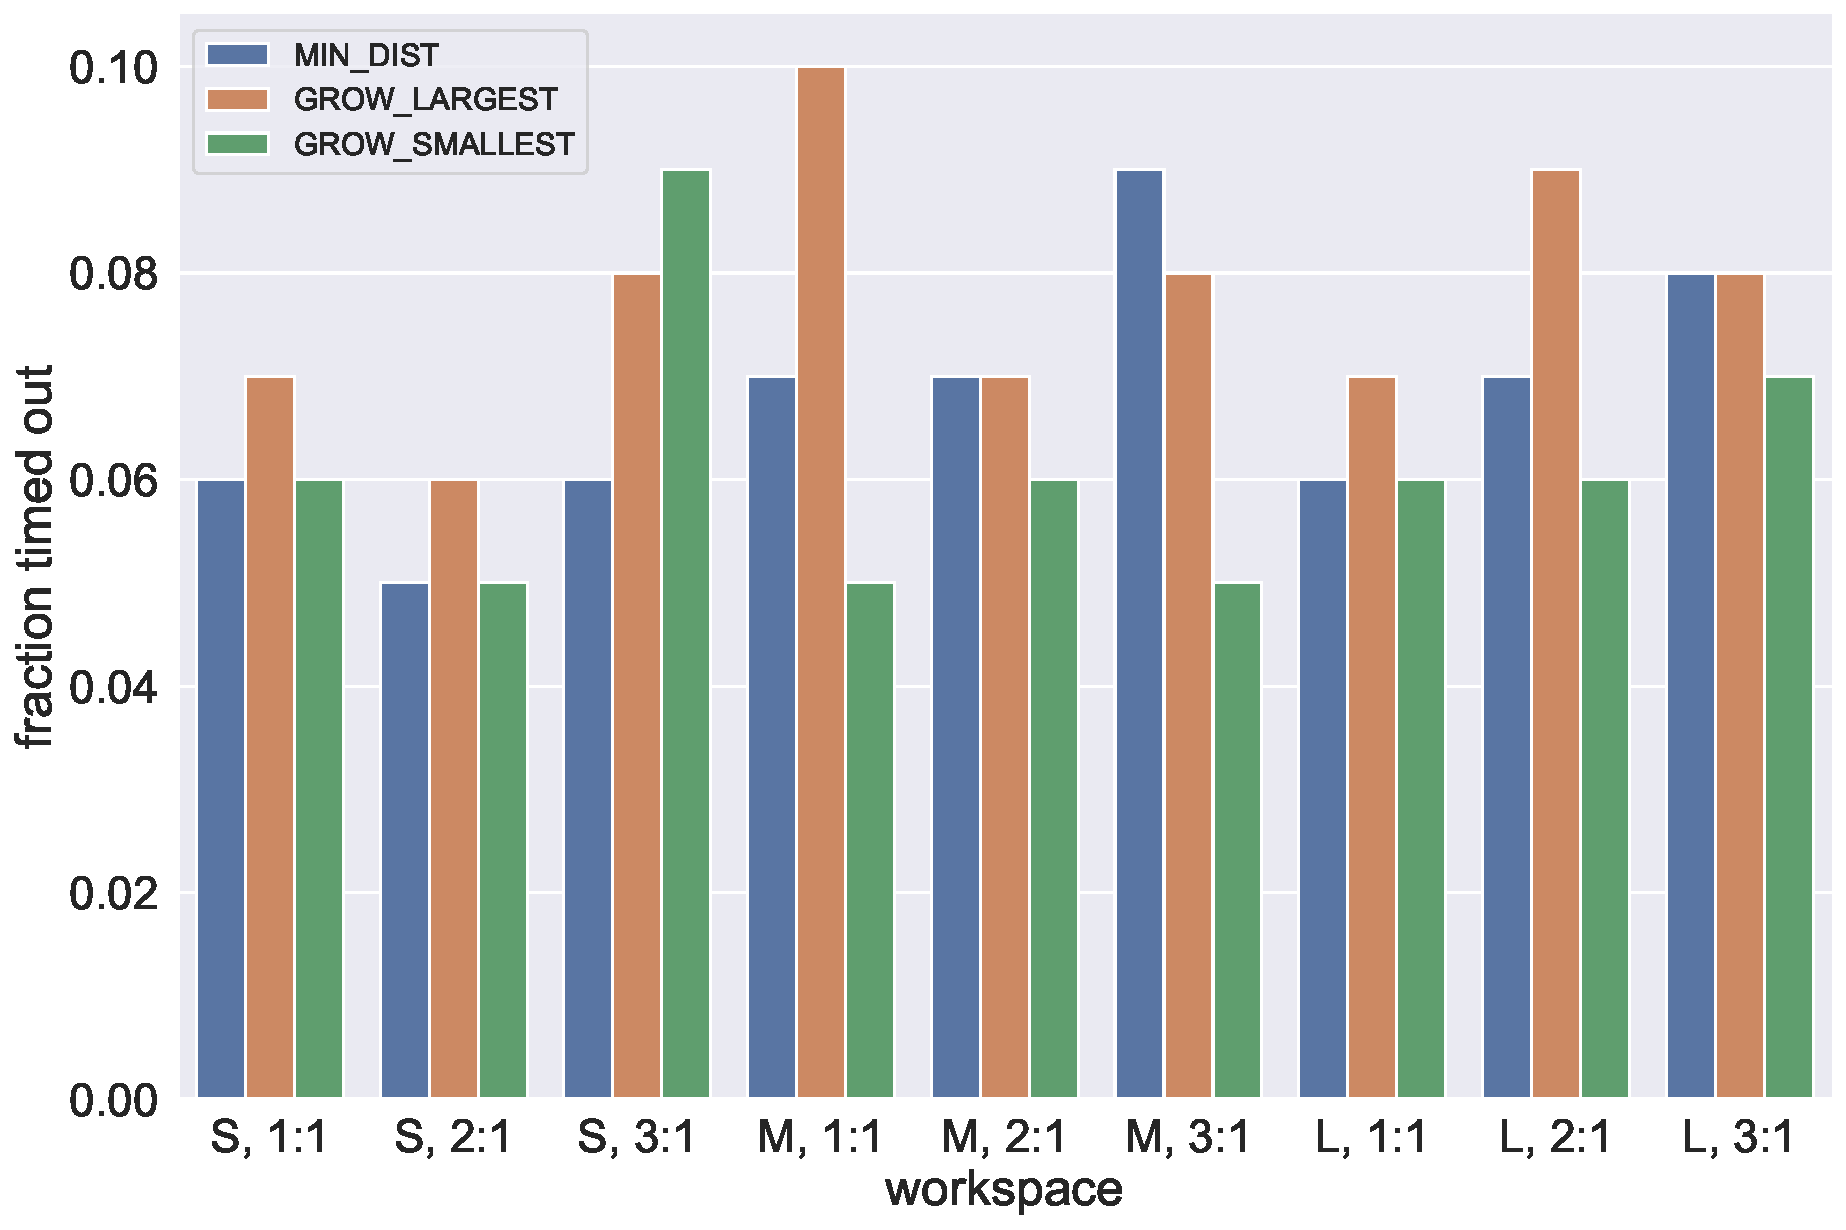
\includegraphics[width=0.9\textwidth]{figures/plots/AFBS_timeout.pdf}
		\caption{Fraction of plans that timed out.}
		\label{fig:AFBS_timeout}
	\end{subfigure}
	\caption[Planning time and fraction timed out for different workspace variations]{Planning time and fraction timed out for different workspace variations listed in \autoref{tab:workspaces}. All option sorting strategies are compared.}
	\label{fig:AFBS_timestats}
\end{figure}

\autoref{fig:AFBS_time} shows the planning time for all workspace variations.
In terms of the size within one class of aspect ration no significant affect can be observed.
Narrowing down the workspace by increasing the aspect ration seems to increase planning time slightly, but for the majority of instances planning time stays under $100$ seconds.
The fraction of timeouts in \autoref{fig:AFBS_timeout} remains constant for all workspaces and the options sorting strategies do not show any difference as well.

\paragraph{Plan Cost} 

\begin{figure}
	\centering
	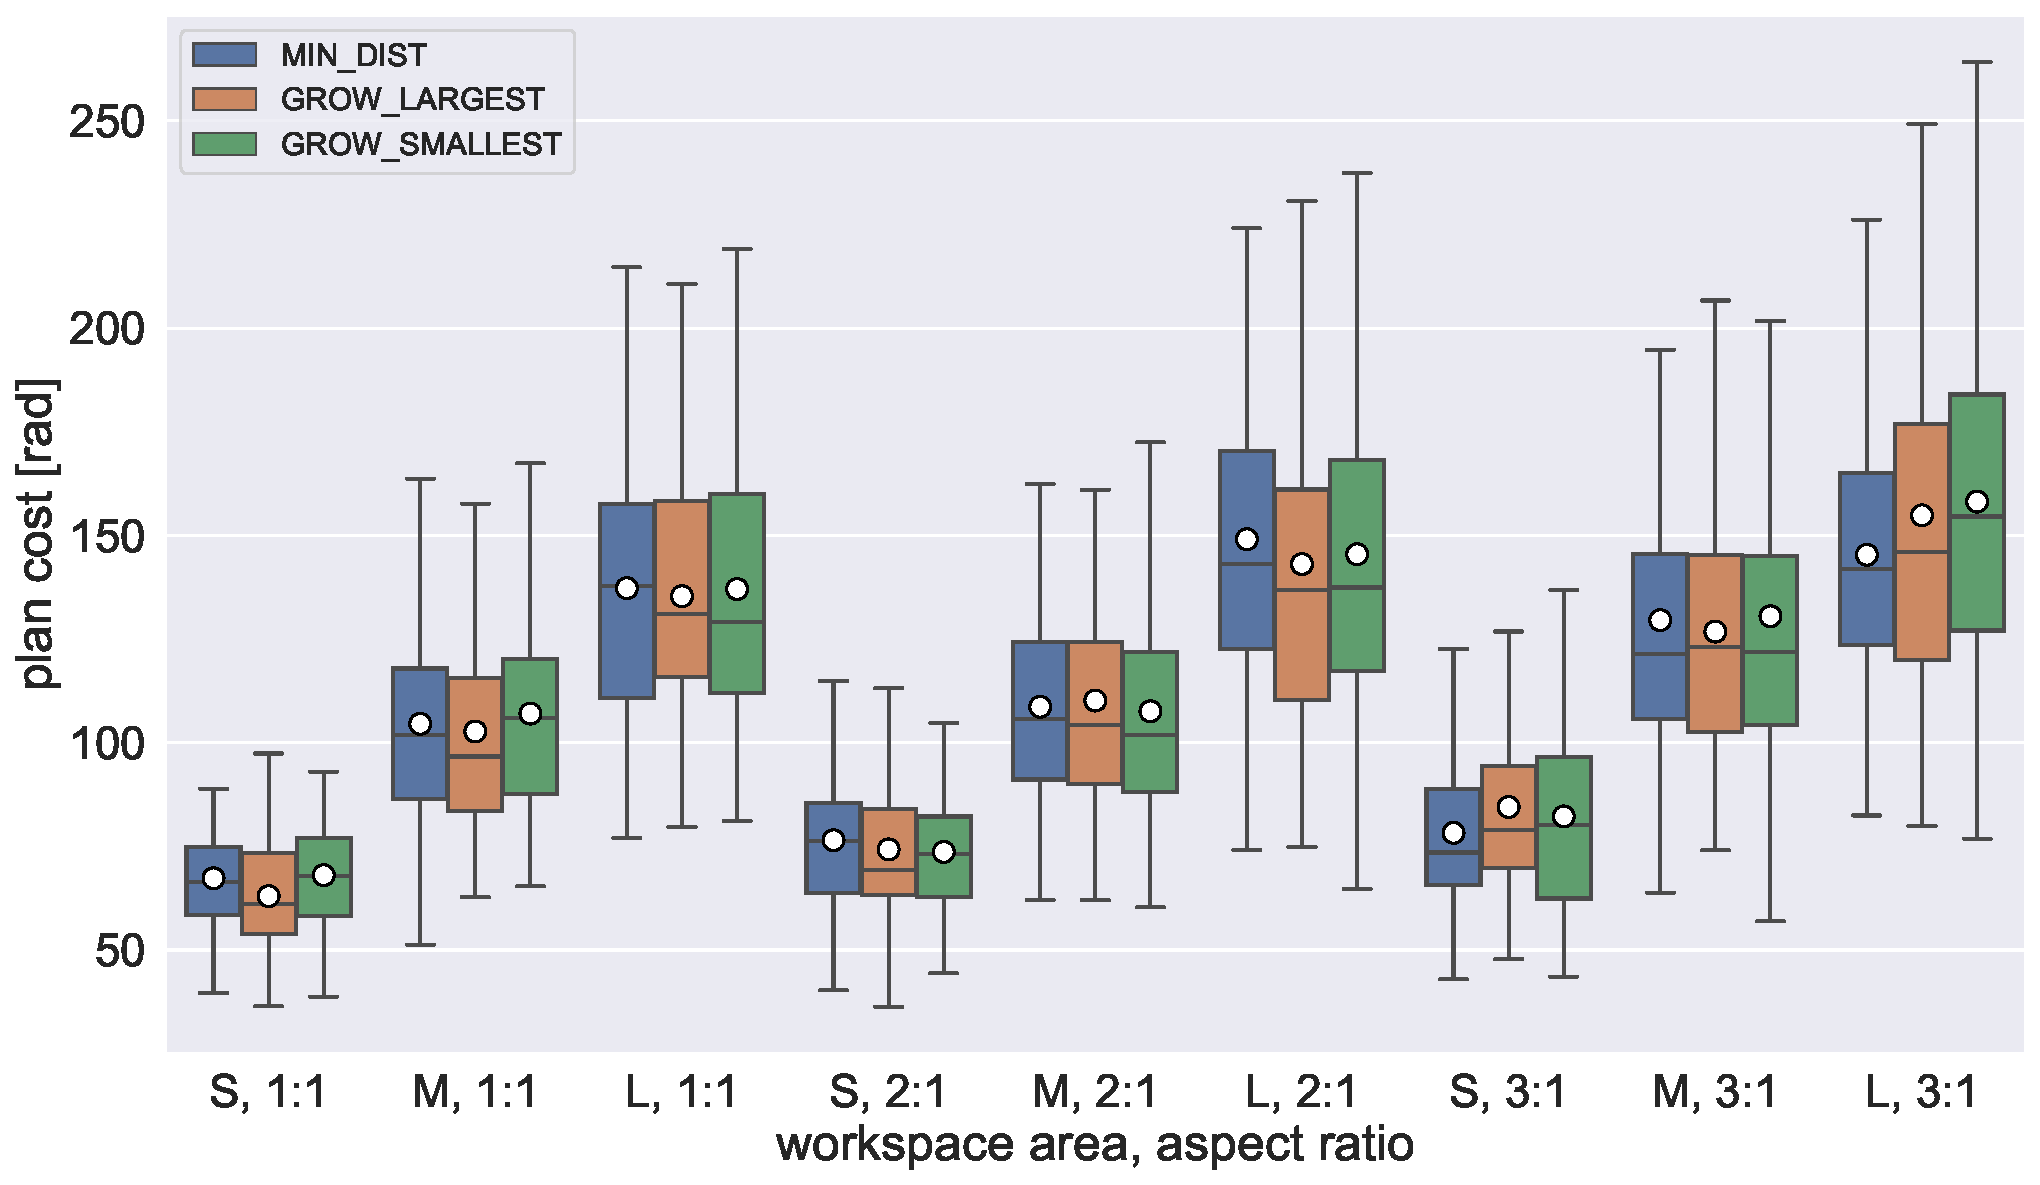
\includegraphics[width=0.9\textwidth]{figures/plots/AFBS_cost.pdf}
	\caption[Plan cost for different workspace variations]{Plan cost in radians of successful plans for different workspace variations with varying areas and aspect ratios. All option sorting strategies are compared.}
	\label{fig:AFBS_cost}
\end{figure}

It is not surprising that the distribution of rotational cost, presented in \autoref{fig:AFBS_cost}, increases with bigger workspace areas.
Cubes and walls are further apart, which results in more pivot walking steps necessary to assemble polyominoes.
With in a class of same size, increasing the aspect ratio results in slightly more rotational cost as well.





\section{Assembly for Red and Blue Cube Ratio}
\label{sec:AFNR}

We examined the affect of red and blue cube ratio on planning time.
For this we increased the number of red cubes $0 \leq n_\textit{red} \leq \lfloor \frac{n}{2}\rfloor$ while keeping the target polyomino size fixed at $n = 10$.
With $n_\textit{red} = 0$ only north-south connections allow the creation of just a vertical line polyomino.
$n_\textit{red} = \lfloor \frac{n}{2}\rfloor$ holds the biggest variety of polyomino shapes.
To exclude the influence of varying polyomino shapes on the experiment, the shape is set to a $10 \times 1$ polyomino.
$\lfloor \frac{n}{2}\rfloor < n_\textit{red} \leq n$ is equal to $0 \leq n_\textit{blue} \leq \lfloor \frac{n}{2}\rfloor$.
Conducting the experiment with $n_\textit{red}$ or $n_\textit{blue}$ in equivalent.
The patterns of red and blue cubes within the $10 \times 1$ polyomino and the initial configurations are randomly generated in a workspace of size $50 r_C \times 50 r_C$.
For each $n_\textit{red}$ $100$ samples were taken.

\paragraph{Planning Time}

\begin{figure}
	\centering
	\begin{subfigure}[b]{\textwidth}
		\centering
		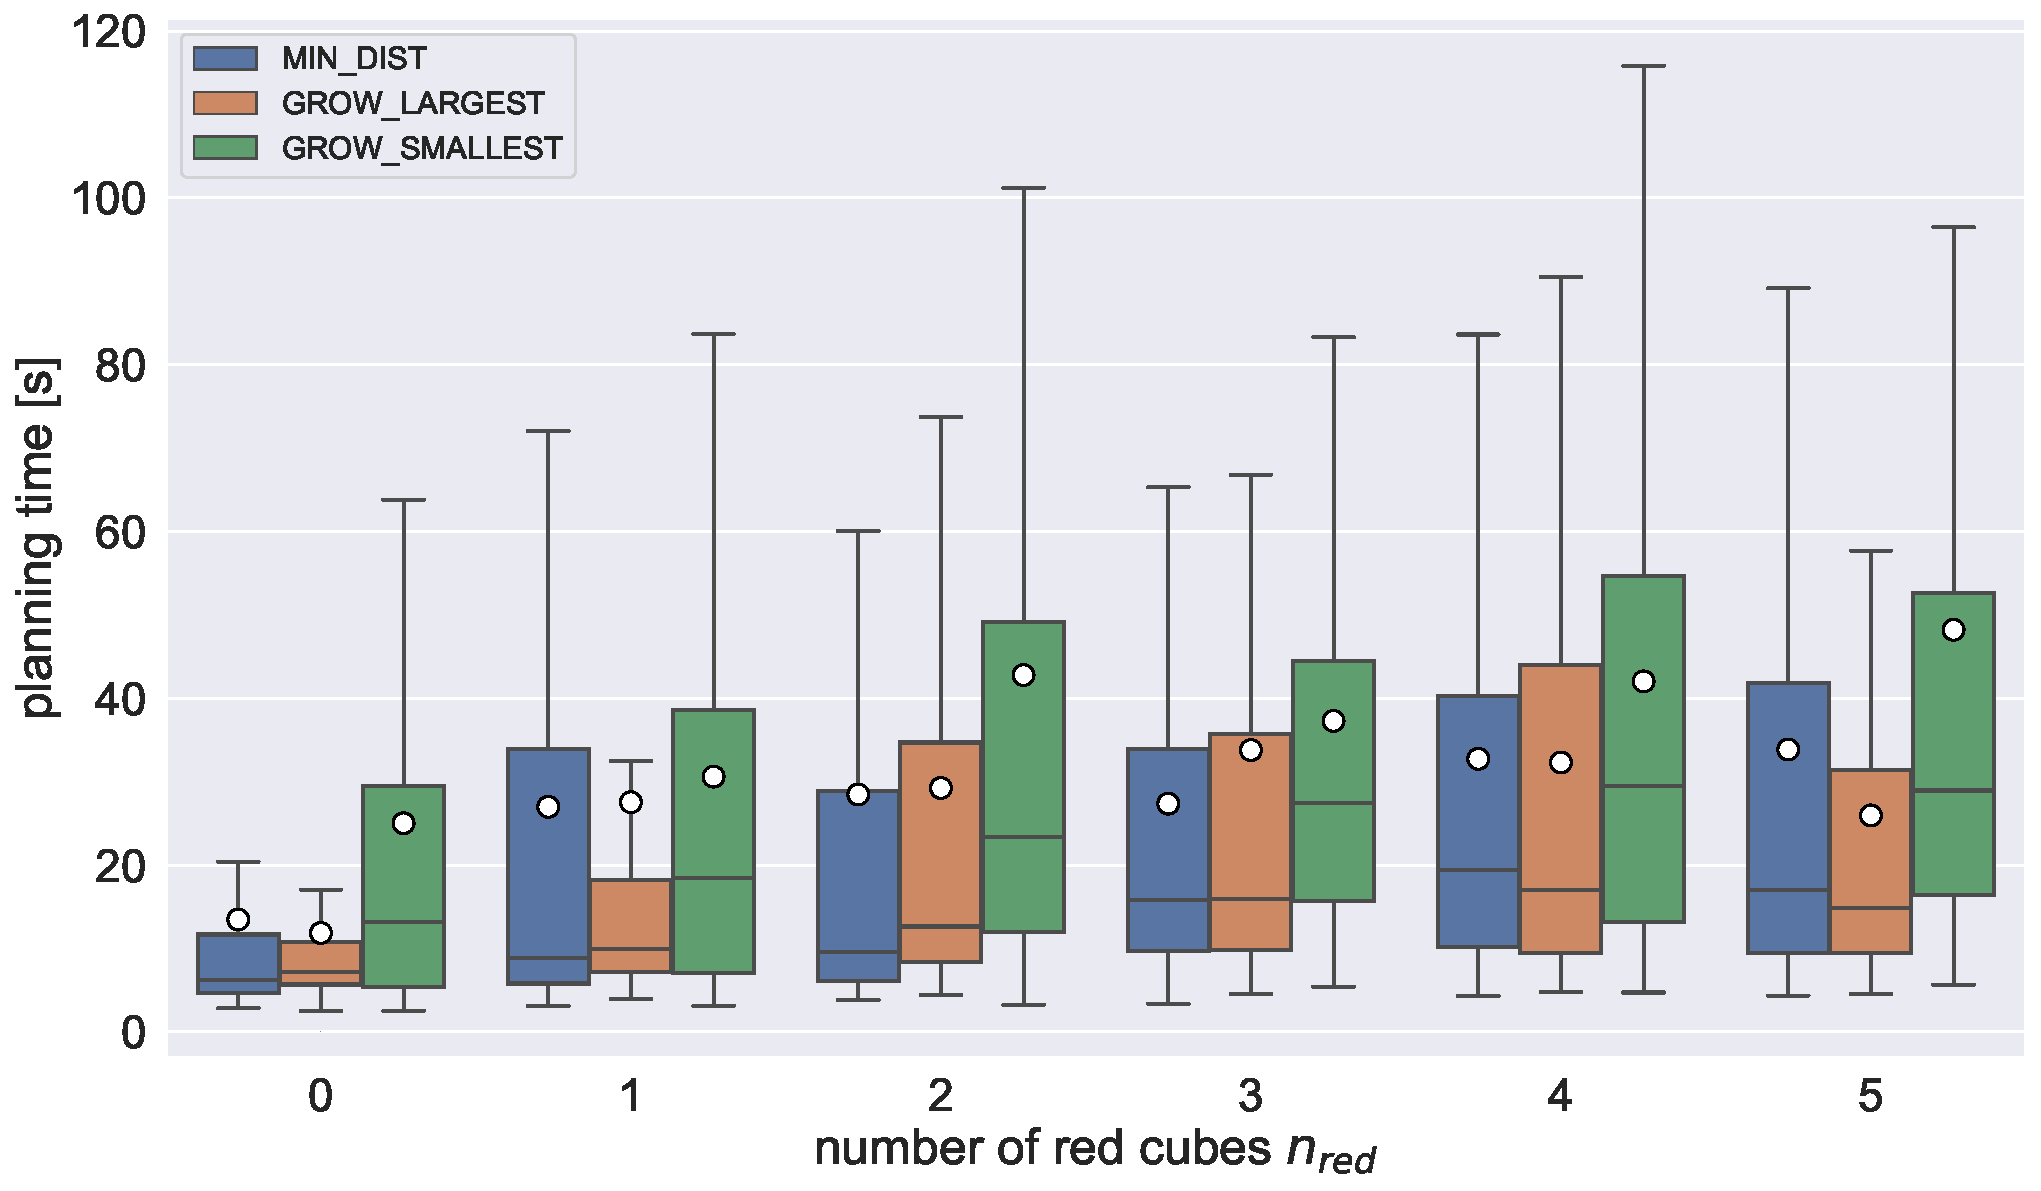
\includegraphics[width=0.9\textwidth]{figures/plots/AFNR_time.pdf}
		\caption{Planning time in seconds. Only plans that did not time out are shown.}
		\label{fig:AFNR_time}
	\end{subfigure}
	
	\begin{subfigure}[b]{\textwidth}
		\centering
		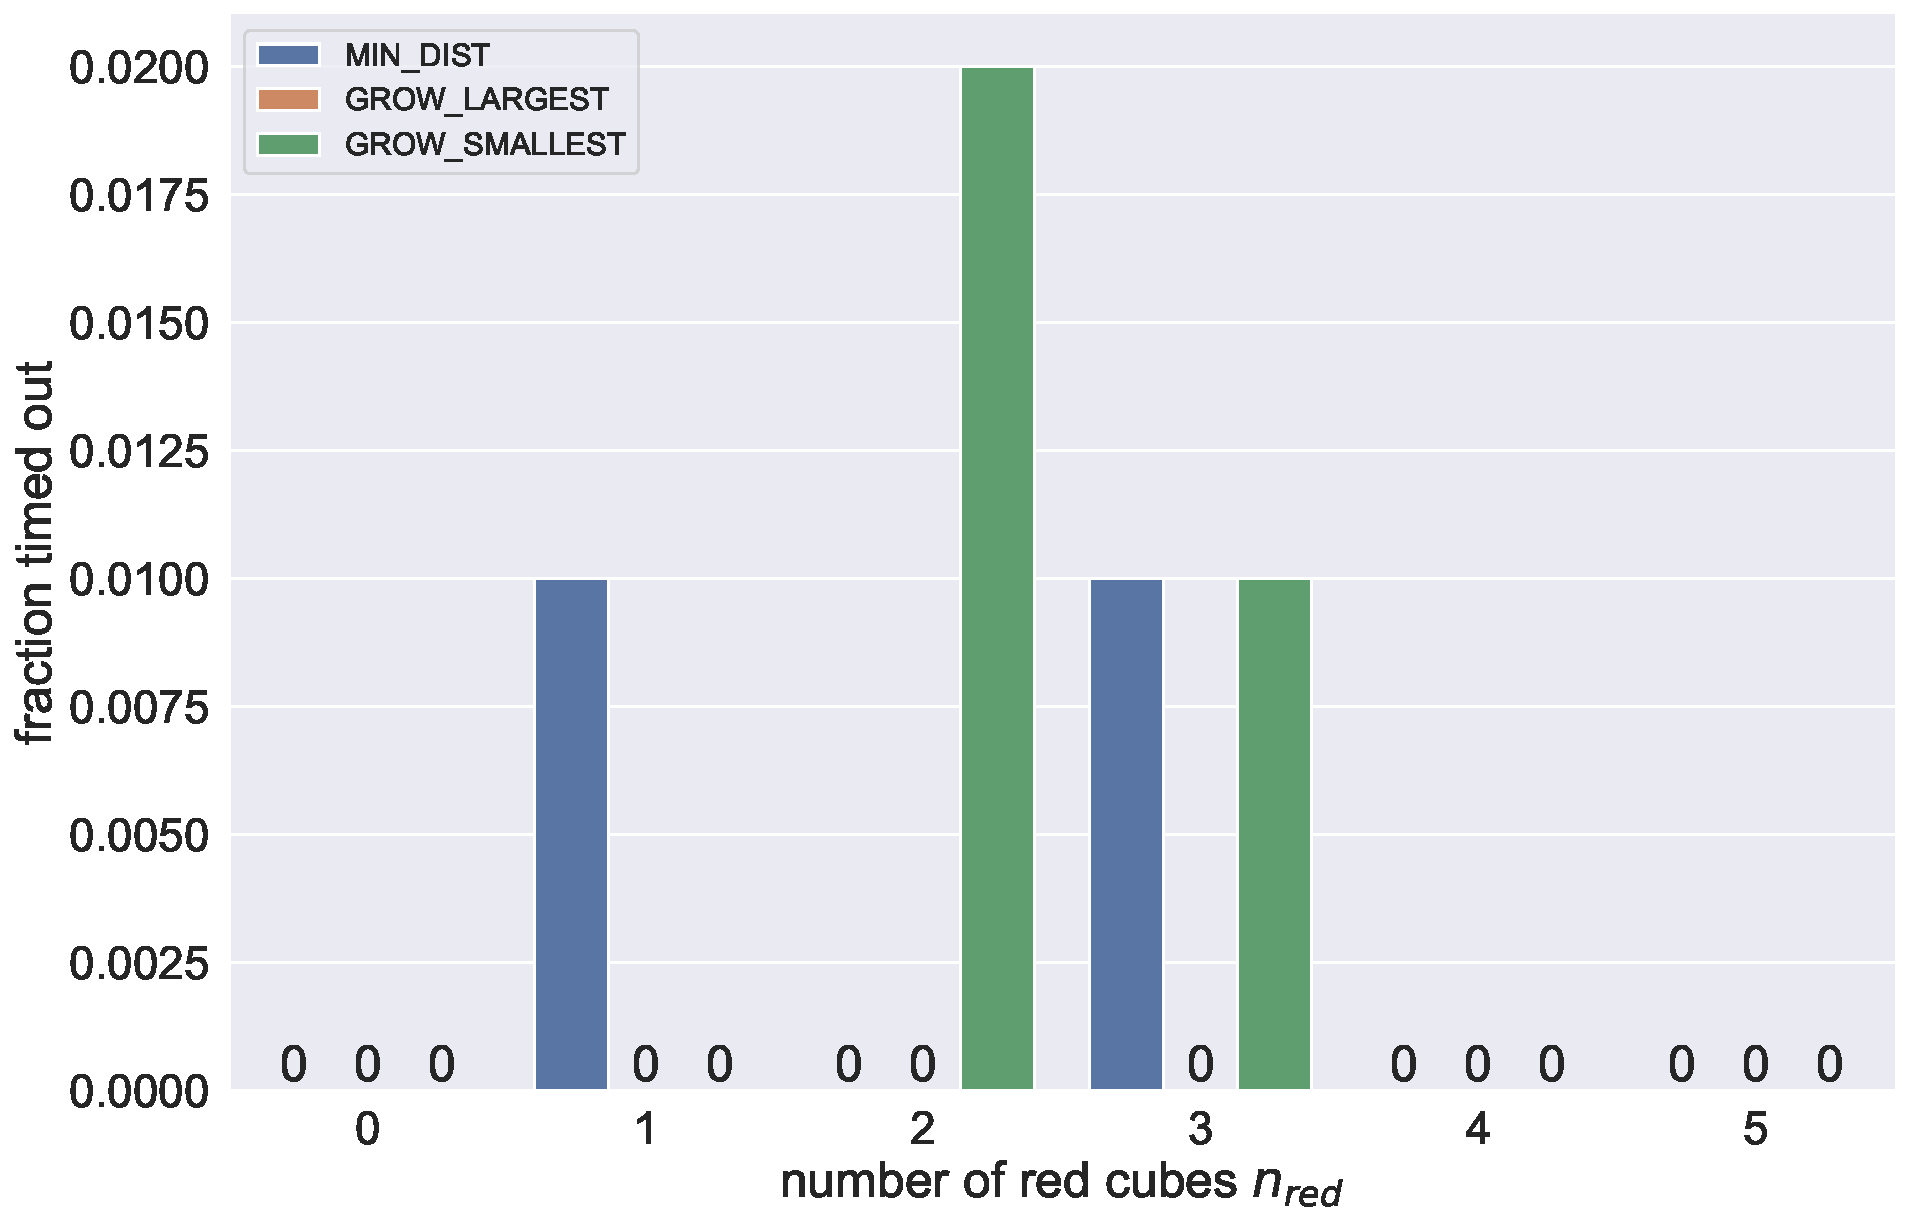
\includegraphics[width=0.9\textwidth]{figures/plots/AFNR_timeout.pdf}
		\caption{Fraction of plans that timed out.}
		\label{fig:AFNR_timeout}
	\end{subfigure}
	\caption[Planning time and fraction timed out for number of red cubes]{Planning time and fraction timed out for different numbers of red cubes $n_\textit{red}$. All option sorting strategies are compared.}
	\label{fig:AFNR_timestats}
\end{figure}

\autoref{fig:AFNR_time} shows the distribution of planning time for this experiment.
By increasing $n_\textit{red}$ from $0$ to $1$ a clear increase in planning time is visible.
With only blue cubes every cube can be placed everywhere in the polyomino.
By introducing one red cube position becomes important.
Further increasing the number of $n_\textit{red}$ does not affect planning time significantly.
For these vertical straight line polyominoes growing the smallest component performs slightly worst than the other two option sorting strategies.
The fraction of timeouts presented in \autoref{fig:AFNR_timeout} is under $2\%$ for all $n_\textit{red}$. 



